\documentclass[10pt,twocolumn]{article}

\usepackage{times}
\usepackage{fullpage}

\usepackage{booktabs}  % for \midrule
%\usepackage{subfigure}
\usepackage{balance}
\usepackage{graphicx}
\usepackage{xspace}
%\usepackage{pslatex}
%\usepackage{pifont}
%\usepackage{multirow}
%\usepackage{array}
%\usepackage{booktabs}
%\usepackage{cite}
\usepackage{url}
%\usepackage{cancel}
\usepackage{color,colortbl}
%\usepackage{microtype}
%\usepackage{textcomp}% http://ctan.org/pkg/textcomp
\usepackage{tabularx}
\usepackage{framed}
\usepackage[]{algorithm2e}
\SetAlFnt{\small}
\SetAlCapFnt{\small}
\usepackage{algorithmic}

\usepackage{listings}
%\usepackage{scrextend}
%\usepackage{mathtools}
\usepackage{pbox}
\usepackage{amsmath}

\let\labelindent\relax
\usepackage{enumitem}

\usepackage{tikz}
\usetikzlibrary{arrows,automata}
\usetikzlibrary{calc,positioning}
\usepackage{lipsum,adjustbox}


%\usepackage{tikz}
%\usepackage{decorations.pathmorphing}
%\usepackage{assymb}

\usepackage[labelfont=bf]{caption}

\usepackage{caption}
\usepackage{subcaption}
\usepackage{cleveref}
\captionsetup[subfigure]{subrefformat=simple,labelformat=simple}

%\theoremstyle{plain}
\newtheorem{theorem}{\bf{Theorem}}%[section]
\newtheorem{lemma}[theorem]{\bf{Lemma}}
\newtheorem{corollary}[theorem]{\bf{Corollary}}
\newtheorem{proofl}[theorem]{\bf{Proof}}
\newtheorem{proposition}[theorem]{\bf{Proposition}}

%\theoremstyle{definition}
\newtheorem{definition}{\bf{Definition}}%[section]
\newtheorem{observation}{\bf{Observation}}%[section] 

%\theoremstyle{remark}
\newtheorem{example}{\bf{Example}}
\newtheorem{notation}{\bf{Notation}}
\newtheorem{fact}{\bf{Fact}}

\usepackage{listings}
%%\usepackage{listings-golang}
\usepackage{color}

%\usepackage{sectsty}
%\sectionfont{\fontsize{12}{15}\selectfont}


\newcommand\mypara[1]{\vspace{.3em}\noindent\textbf{#1}}
\newcommand{\urlwofont}[1]{\urlstyle{same}\url{#1}}


%%%%%%%%%%%%%%%%%%%%%%%%%%%%%%%%%%%%%%%%
% Useful reviewing/feedback annotations
\usepackage{ifthen}
\usepackage[normalem]{ulem} % for \sout
\usepackage{xcolor}
\usepackage{amssymb}

\newcommand{\ra}{$\rightarrow$}
\newboolean{showedits}
\setboolean{showedits}{true} % toggle to show or hide edits
\ifthenelse{\boolean{showedits}}
{
	\newcommand{\ugh}[1]{\textcolor{red}{\uwave{#1}}} % please rephrase
	\newcommand{\ins}[1]{\textcolor{blue}{\uline{#1}}} % please insert
	\newcommand{\del}[1]{\textcolor{red}{\sout{#1}}} % please delete
	\newcommand{\chg}[2]{\textcolor{red}{\sout{#1}}{\ra}\textcolor{blue}{\uline{#2}}} % please change
}{
	\newcommand{\ugh}[1]{#1} % please rephrase
	\newcommand{\ins}[1]{#1} % please insert
	\newcommand{\del}[1]{} % please delete
	\newcommand{\chg}[2]{#2}
}

\newboolean{showcomments}
\setboolean{showcomments}{true}
% \setboolean{showcomments}{false}
\newcommand{\id}[1]{$-$Id: scgPaper.tex 32478 2010-04-29 09:11:32Z oscar $-$}
\newcommand{\yellowbox}[1]{\fcolorbox{gray}{yellow}{\bfseries\sffamily\scriptsize#1}}
\newcommand{\triangles}[1]{{\sf\small$\blacktriangleright$\textit{#1}$\blacktriangleleft$}}
\ifthenelse{\boolean{showcomments}}
%{\newcommand{\nb}[2]{{\yellowbox{#1}\triangles{#2}}}
{\newcommand{\nbc}[3]{
 {\colorbox{#3}{\bfseries\sffamily\scriptsize\textcolor{white}{#1}}}
 {\textcolor{#3}{\sf\small$\blacktriangleright$\textit{#2}$\blacktriangleleft$}}}
 \newcommand{\version}{\emph{\scriptsize\id}}}
{\newcommand{\nbc}[3]{}
 \renewcommand{\ugh}[1]{#1} % please rephrase
 \renewcommand{\ins}[1]{#1} % please insert
 \renewcommand{\del}[1]{} % please delete
 \renewcommand{\chg}[2]{#2} % please change
 \newcommand{\version}{}}
\newcommand{\nb}[2]{\nbc{#1}{#2}{orange}}

\definecolor{ibcolor}{rgb}{0.4,0.6,0.2}
\newcommand\iv[1]{\nbc{IB}{#1}{ibcolor}}
\usepackage{wasysym}
\newcommand\yesml[1]{\nbc{ML {\textcolor{yellow}\sun}}{#1}{mircolor}}

\definecolor{sgcolor}{rgb}{0.2,0.0,0.5}
\newcommand\sg[1]{\nbc{SG}{#1}{sgcolor}}

\definecolor{samcolor}{rgb}{0.2,0.4,0.2}
\newcommand\sam[1]{\nbc{SC}{#1}{samcolor}}

\definecolor{hccolor}{rgb}{0.21,0.54,0.84}
\newcommand\hc[1]{\nbc{HC}{#1}{hccolor}}

\definecolor{ideacolor}{rgb}{1.0,0,0.5}
\newcommand\idea[1]{\nbc{IDEA}{#1}{ideacolor}}


\definecolor{abstractcolor}{rgb}{0.0,0.5,1.0}
\newcommand\rabstract[1]{\nbc{ABSTRACT}{#1}{abstractcolor}}

\definecolor{introcolor}{rgb}{0.0,1.0,0.5}
\newcommand\rintro[1]{\nbc{INTRO}{#1}{introcolor}}

\definecolor{papercolor}{rgb}{1.0,1.0,0.0}
\newcommand\rpaper[1]{\nbc{PAPER}{#1}{papercolor}}

\definecolor{multicolor}{rgb}{1.0,0,0}
\newcommand\rmulti[1]{\nbc{MULTI}{#1}{multicolor}}

% Todo Command
\definecolor{todocolor}{rgb}{0.9,0.1,0.1}
\newcommand{\todo}[1]{\nbc{TODO}{#1}{todocolor}}


%%%%%%%%%%%%%%%%%%%%%%%%%%%%%%%%%%%%%%%%


\begin{document}

\title{Cuckoo for Clients: Disaggregated Cuckoo Hashing}
%\author{WORDS '21 Submission \#3}
% \author{Stewart Grant and Alex C. Snoeren\\ UC San Diego}
\author{ATC '24 Submission \#820}
\date{}

\maketitle

\section*{Abstract}

Memory disaggregation promises high resource utilization,
and efficient resource sharing. However designing fully
disaggregated systems remains challenging due to complex
serialization, high latency, and failures. Key-value store 
indexes often adopt a partially disaggregated approach
where writes to the index are routed through a CPU for
serialization, while reads are made directly to memory.
Fully disaggregation assumes no such CPU and must serialize
writes entirely with clients.

In this paper we describe the first fully disaggregated
lock based cuckoo hash. Prior work avoids locks in favor of
optimistic concurrency as locks can have large critical
sections and complex failures. We show that that with
careful design locks can have higher performance than
opportunistic algorithms and recover from failures quickly.
We develop a locality based hashing algorithm which enables
fast reads, and efficient locking. We compare our
performance against state of the art key value stores and
show gains on an YCSB benchmarks against all systems
achieving between 1.4x to 10x on write heavy workloads and
1.3x to 2.2x on read heavy workloads.


% with careful data structure and protocol design, as well as
% the architecture of modern RDMA NICs traditional locking
% strategies can perform better than state of the art
% optimistic concurrency algorithms. We demonstrate this
% through the design of a remote memory key value store based
% on cuckoo hashing. Our cuckoo hashing algorithm (rcuckoo)uses dependent,
% rather than independent hash functions to increase the
% probability that both hashes of a key will be
% close in the hash table. This locality enables fast lock
% acquisition and release. We demonstrate that rcuckoo
% outperforms optimistic concurrency algorithms by 2x in
% terms of throughput and up to a 2x improvement on read
% latency.

\section{Introduction}
\label{sec:intro}

Key/value stores remain a fundamental building block of modern
scale-out service architectures.  Recent trends in primary storage
technologies, however, are pushing operators to consider ever-more
disaggregated designs for their in-memory storage systems.
Concretely, increases in CPU core counts coupled with stagnating DRAM
density has led to an increased interest in remote memory tiers, where
some portion of memory is connected to the server over a network.
Moreover, once disaggregated, memory can---in theory, at least---be
pooled to achieve greater cost and power efficiencies.  A key
challenge facing the widespread depolyment of fully disaggregated
memory pools, however, is the current inability to sustain
high-throughput, low-latency lookups in the face of 
concurrent updates and/or client failures.
%and high access latencies.
%---e.g., 20$\times$ in the case of Ethernet-based RDMA.

While cache-coherent technologies like CXL are beginning to enter the
marketplace, RDMA remains the commodity option for large-scale
in-memory key/value stores.
%% % made DRAM a scarce resource. In response data center
%architects have % proposed resource disaggregation to
%improve resource utilization, % scalability and efficiency
%as well as increase per-core access to % memory.
%Disaggregation calls for the partitioning of a servers %
%resources into distinct pools (compute, memory, storage, %
%accelerators), which are interconnected by a high speed
%network.  In a % fully disaggregated model distinct servers
%house resources such as % memory servers which contain only
%memory, and no collocated CPU for % processing.  DRAM
%capacity is scaling at an ever decreasing rate. As such the
%demand in data centers for high efficiency memory systems
%grows every year to improve memory utilization and sharing.
%Memory disaggregation i.e separating compute and memory
%into large pools is a promising approach to increase a
%CPU's per core memory access beyond what is available in a
%single machine while simultaneously decreasing per machine
%memory stranding.
%
%% Full disaggregation is challenging as it requires new
%system % designs to cope with the additional network
%latency.  For % example accessing intra-rack remote DRAM
%has a 20x (50ns to % 1us) overhead in relation to local
%memory. Cores sharing % remote memory must suffer a
%proportionally high cost for % synchronization when sharing
%pools of memory.  Many prior disaggregated systems have
%eschewed sharing for static partitioning to avoid the high
%overheads~\cite{ reigons,blade-server,legoos}.
Most existing RDMA-based systems only partially deliver on the
disaggregated vision, requiring one or more CPU cores to be collocated with
remote memory to implement traditional access semantics~\cite{erpc,herd,pilaf,cell,clover,sherman}.
%%  ~\cite{clover}. These designs are conceptually % close
%to prior work on RDMA key value stores which gain %
%performance benefits from having some operations use %
%one-sided RDMA verbs\footnote{one-sided verbs are %
%disaggregation compliant as they do not require a CPU on
%the % receiver side during operation} % %% % % While highly
%performant these approaches do not conform to % fully
%disaggregated designs.
%
%to remote memory are approximately 20x that of local DRAM
%(50ns to 1us) which severely increases the cost of
%synchronizing shared data structures among many CPU's
%across multiple machines. Traditional and partially
%disaggregated key-value serialize updates with a CPU
%collocated with
%memory~\cite{memcached,herd,erpc,pilaf,cell,clover}(\todo{check
%Sherman}). This approach does not meet the requirements of
%full disaggregation in which memory is a passive resource.
%In the fully disaggregated setting serialization is
%achieved entirely with a client based protocol. 
%
The few systems that realize full disaggregation must rely upon one-sided RDMA atomic
operations (e.g., compare-and-swap) to resolve data
races~\cite{rolex,fusee,race} which constrains their design.
%suffer from the limited scope of such operations.
Specifically, RDMA atomic operations can act upon at most 64 contiguous bits
of memory at a time, forcing existing systems to employ
multi-stage datastructures to support practical key/value sizes, resulting in multiple-RTT reads and expensive write operations.

Due to the limited width of RDMA atomic operations, existing fully disaggregated systems rely upon compact index
structures that localize key operations and maintain values in
entirely separate memory regions, necessitating multiple RDMA
operations and network round trips.
%even in the absence of contention.
Moreover, given the dominance of read-heavy
workloads~\cite{rocks-db-workload,facebook-memcached}, these systems
tend to eschew locks in favor of optimistic update approaches that
lead to poor performance under even modest contention.  Our tests show the performance of even the highest-performing existing systems collapses beyound 128 clients under a YCSB-B (5\% update) workload.

%optimistically update the index with pointers to
%enable lock-less reads avoid locking overheads and failures with
%visible partial writes.  Unfortunately, optimistic approaches can
%perform worse under high contention and demand indirect reads, leading
%to an awkward trade space.
%
%% These approaches either use optimistic
%% concurrency, or assume that most clients are collocated and
%% can resolve their lock acquisitions in local memory.
%% Optimistic approaches using RDMA atomics are limited by the
%% width of the atomic instruction (64 bits for compare and
%% swap). 64 bits is often too small to encapsulate a full
%% key-value update. The result is that optimistic approaches
%% require more round trips to remote memory to complete their
%% operations. These approaches have dismissed lock based
%% approaches outright as the size of their critical sections
%% can bottleneck performance, and  the cost of acquiring and
%% releasing locks (at minimum two round trips) is often higher
%% than the optimistic approach (two or three round trips).
%
% %concurrent data structures round trips
% Concurrent data structure design for remote memory is hard.
% Access latency to remote memory is high so round trips per
% operation must be minimized to achieve efficiency.
% Serialization is particularly hard because there is no
% centralized serialization point to guard access to remote
% memory. RDMA NIC's provide atomic verbs such as
% compare-and-swap (CAS), but these are by no means a silver
% bullet.  Each atomic request takes a round trip from client
% to server to execute. In the best case lock/unlock requires
% two round trips, if multiple locks are required, or locks
% are contested the number of round trips increases.
%
% %CPU locking vs RDMA
% In traditional key-value stores (Memcached~\cite{memcached})
% the CPU coordinates table access for read, write, and lock
% instructions. In contrast RDMA based Key-value
% stores~\cite{herd,erpc,pilaf} use a mixture of one-sided (no
% CPU) and two-sided (CPU involved) verbs to alleviate the CPU
% bottleneck. Reads are typically one sided to bypass the CPU
% bottleneck~\cite{pilaf,cell} while writes are typically two
% sided so memory-side CPU can orchestrate serialized
% operations (e.g. locking) with main memory access latency
% (50-100ns).  These small access times keep critical sections
% small for CPU based locking, and dramatically increase them
% for one-sided RDMA based locking schemes~\cite{clover,
% Sherman}.
%
%RDMA and cuckoo hashing
In this work we design a fully disaggregated key/value store that
simultaneously delivers low latency and high throughput for read/write
workloads despite the constraints of current RDMA hardware.
Specifically, we facilitate lock-based datastructures by decreasing
the number of round trips required to acquire locks and perform
mutating operations with RDMA atomics.  Our high-performance locks
allow us to employ more sophisticated index structures than prior
systems can support, as their optimistic updates scale poorly with
both increased contention and operation complexity.

\begin{figure*}[t]
    \centering
    \begin{subfigure}{0.3\linewidth}
        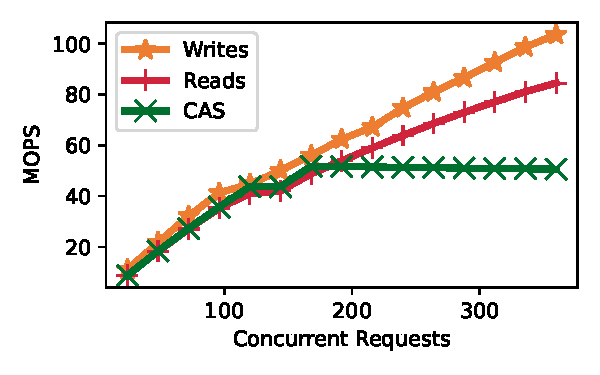
\includegraphics[width=0.99\linewidth]{fig/rdma_concur.pdf}
        % \label{fig:optimistic_failures}
        % \caption{}
    \end{subfigure}
    \begin{subfigure}{0.3\linewidth}
        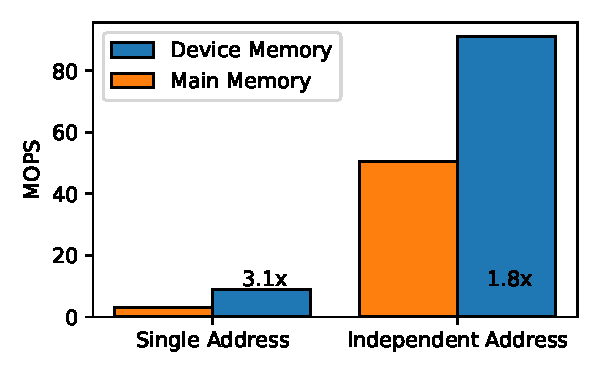
\includegraphics[width=0.99\linewidth]{fig/rdma_cas_throughput.pdf}
        % \label{fig:optimistic_failures}
        % \caption{}
    \end{subfigure}
    \begin{subfigure}{0.3\linewidth}
        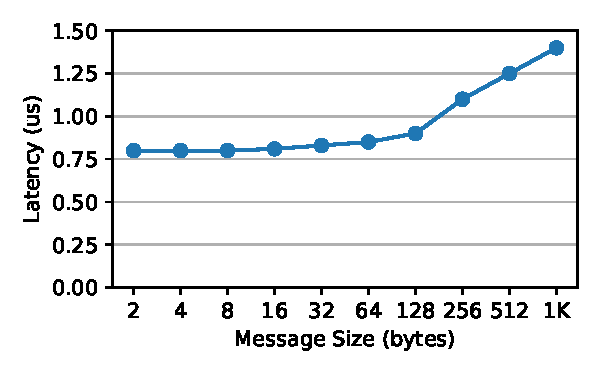
\includegraphics[width=0.99\linewidth]{fig/rdma_latency.pdf}
        % \label{fig:rdma_latency}
        % \caption{}
    \end{subfigure}
    \vspace{-1em}
    \caption{Basic RDMA performance on our testbed.
    \textbf{(a)} (64-bit) main-memory operation performance;
    \textbf{(b)} compare-and-swap (CAS) performance on device and main memory; and
    \textbf{(c)} operation latency as a function of message size~\cite{rdma-latency}.}
    \label{fig:rdma-benchmarks}
\vskip -1em
\end{figure*}

%
We introduce RCuckoo, a fully disaggregated key/value store based on
cuckoo hashing~\cite{cuckoo} that
%delivers high performance using
uses only one-sided RDMA operations.
%At its heart,
RCuckoo builds
around a \emph{dependent hashing} algorithm that makes spatial
locality a tunable parameter.
%
%Locality enables us
%to effectively predict the locks, and rows required to perform
%operations and to set multiple locks with a single atomic
%operation. We design and implement a fast fault tolerance algorithm
%which allows distributed clients to detect and repair failures in the
%table while still issuing millions of operations per second.
%
%%  The core insight of our work is
%% that round trips can be decreased by increasing locality in
%% the table and the size of reads.
%
% Dependent hashing increases the likelihood that
% a key's hash locations will be spatially near one another;
% if locations are close enough, a client can read them both
% with a single RDMA operation.  Of course, the increased
% locality leads to a higher degree of collisions, impacting
% the maximum number of elements which can be inserted into
% the table (i.e., fill factor).  We explore the trade space
% to find the best balance  between performance and fill
% factor. Using this locality we design a dense lock table
% which can fit into RDMA NIC device memory as it provides up
% to 3$\times$ higher performance for contested atomic access.
% Our locking protocol acquires and releases locks in bulk
% using the fewest round trips possible. We use Masked Compare
% and Swap to remove unnecessary contention from out lock
% table.
%
% Using locks rather than CAS to modify our index allows our
% index to support variable sized entries, and allows us to
% inline keys and values directly into the index. Inlining
% entries significantly reduces operation latency. We highly
% optimize inserts into our hash table. Locality between
% key-pairs improves insert locality enabling RCuckoo to both
% find valid cuckoo paths efficiently and acquire all locks for
% insertion in few round trips. We achieve this with a mixture
% of smart caching, searching, and a two stage cuckoo path
% finding algorithm. Finally locality improves reads by using
% single larger reads when key pairs are close, rather than
% multiple smaller reads.
%
% Inserting into a cuckoo hash table normally requires
% acquiring many locks randomly throughout the table,
% dependent hashing clusters lock acquisitions enabling many
% locks to be acquired in a single atomic request. Second, our
% algorithm uses speculative lock acquisition. Locks are
% acquired in bulk based on a local cache of the remote index.
% Once locks are held a second search on synchronized locked
% data is performed to ensure a correct insertion. Third we
% use locality to improve both read and search speeds. We find
% that using a single large read over two smaller reads
% improves throughput when key locations are known to be
% physically close.
%
% \sg{Sherman uses masked compare and swap as well as device
% memory, we might use it better but it's hard to claim a
% contribution here.}
%
%Prior work suggests many important real-world workloads are
%read-heavy, with most objects being small.
RCuckoo employs a set of
complimentary techniques that leverage this enhanced locality to deliver higher performance than any prior
disaggregated key/value store while gracefully handling client
failures:

\begin{itemize}
\item{\textbf{Deterministic lock-free reads.}  Cuckoo hashing ensures
  an entry is always located in one of two memory locations which can be
  read in parallel.}

\item{\textbf{Space-efficient locks} allow clients to acquire necessary 
  locks in a single RDMA operation in most cases.}

\item{\textbf{Client-side caching} enables accurate cuckoo-path
  speculation to improve insert performance.}

\item{\textbf{Leased lock acquisitions} allow clients to detect
  and recover from client failures using timeouts.}
\end{itemize}

%% message round-trips for both reads and writes,
%% improving performance for small-object reads and significantly
%% improving writes.


\noindent Combined with a datastructure design that facilitates
aggressive batching of RDMA operations, these techniques enable
RCuckoo to limit the number of round trips required for all key/value
operations.  In the common case, reads execute in one or two round
trips (for small and large value sizes, respectively), uncontested
updates and deletes require two round trips, and the median insert
operation involves only two round trips---although the expected number
increases as the table fills.

On our testbed,
RCuckoo delivers comparable or higher performance on small values across the standard set  of YCSB benchmarks than all of the existing disaggregated
key/value stores we consider.  Concretely, with 320 clients RCuckoo
delivers up to a 2.5$\times$ throughput improvement on read-intensive
(YCSB-B) workloads and up to 7.1$\times$ their throughput on
write-intensive (YCSB-A) workloads.  Moreover, RCuckoo's
performance remains high despite 100s of
clients failing per second.


\section{Background}
\label{sec:background}

Disaggregated Key-value stores are the highest performance technology for sharing disaggregated
memory with a lineage in RDMA key-value stores. In this section we will provide a background on
existing Disaggregated key values stores and their relationship to prior RDMA KVS. Additionally we
will describe the technological and algorithmic challenges in the design of these systems.


% Key/value stores have long used RDMA to accelerate
% performance~\cite{farm,memc3,erpc,herd,faast,mica,pilaf,cell,storm}.  These systems strike a careful
% balance between directly accessing remote memory with one-sided RDMA requests and serializing
% mutating operations at a server-side CPU.  Cuckoo~\cite{cuckoo} and hopscotch~\cite{hopscotch}
% hashing are popular choices in this space because clients can calculate the location of keys without
% needing to consult the server and potentially perform lock-less reads with
% RDMA~\cite{farm,pilaf,cuckoo}.

\subsection{Disaggregated Key-Value Stores}

The primary difference between disaggregated KVS and prior RDMA KVS is that the former assumes that
servers do not have a CPU capable of serializing requests. Precursor RDMA KV stores achieved
performance by striking a delicate balance between CPU-bypass one-sided RDMA operations and
CPU-serialized two-sided operations~\cite{farm,herd,pilaf,cell,storm}. Disaggregated KVS must only
use one-sided operations even when performing complex operations like insertions which may require
many operations on a hash tables index to resolve collisions.

In general the performance of a disaggregated key-value store hinges on the performance of their
serialization mechanism for writes. Achieving fast consistent writes with one-sided RDMA is hard due
to the limited RDMA atomic interface. Hash indexes are carefully designed around around 8-byte
atomic compare-and-swaps (CAS). Because RDMA atomic writes have a small fixed width a common design
choice for unordered KVS is to use out-of-place optimistic updates~\cite{race,fusee,ditto}. In this
design pattern a hash table index contains 8-byte atomic entires which point to an uncontested
\textit{extent} region containing the actual data. This design pattern has the advantage that the
critical section of a write is only the duration of an RDMA CAS and that client failures do not
effect the state of the index (i.e no locks held). The tradeoff is that index information is highly
limited. Of the 64 bits 48 are used for a pointer typically leaving only 16 bits for data like the
key of the entry or the entries size. This leads to additional round trips to check for a keys
presence or limitations in the size of values an entry can support~\cite{race,fusee}.

KVS with complex data structures like B-Trees or Radix Trees~\cite{Sherman,smart} can't condense the
complexity of their update into 8bytes and must rely on locks to provide mutual exclusion on all or
part of their updates. The advantage of locks is that these structures support inline updates and
thus faster reads, at the cost of expensive writes. Because of locking the cost of contention is
high especially as updates require multiple round trips which inflate critical section size. Thus
these systems rely on the assumptions that many clients are colocated so their writes can be
combined.

While locks are typically regulated for disaggregated KVS with complex data structures they are also
commonly used on hash tables that require multiple inline updates such as Cuckoo and hopscotch
hashes which dominated RDMA KVS research.

This RDMA fact leads to a common design
pattern, KV indexes consist of 64 bit atomic entries that point to data stored in uncontended
memory. This pattern leads to suboptimal data accesses as the condensed nature of the 64 bit entry
usually contains a 48 bit pointer leaving only 16 bits for metadata. Data like the size of the true
entry, and its key are stored in 16 bit compressed digests. This means that reads require at least
two round trips to recover an entry or even validate its existence. In general this design pattern
leads to simplified hash table designs which can not support complex metadata. Established high
performance RDMA hash tables like Cuckoo and hopscotch hashes can’t be implemented with this
strategy as they require locks on multiple entries of the index rather than a single atomic update.

Historically network bandwidth has limited KV store throughput more than operation rate. For
instance a connectx3 nic at 40GBPs can process 75 million packets per second would bottleneck at
only 5MOPS making 1K reads. Similarly at these lower packet rates the effects of contention on
skewed distributions are not as noticeable. As bandwidths get higher (400GBPs+) latency and
contention, rather than bandwidth will become the primary scalability bottleneck. To this end we
focus on small key workloads which are limited by round trip access latency and contention and not
bandwidth. We make specific design choices which reduce round trip times at the cost of bandwidth.

Figure~\ref{fig:rdma-benchmarks}(a) shows the tradeoff in round trip time for RDMA reads of
increasing size. Critically the round trip time of a 1KB packet is lower than the latency of issuing
two dependent small packets.  The implication is that performance can be gained if a single large
packet can complete the work of two dependent smaller messages. Figure~\ref{fig:rdma-benchmarks}(b)
shows the performance overheads of using an extent based design on small key-value pairs. Inlined
values are read directly from the index while all other values are read from indirect storage. Here
client caching is turned on and clients optimistically read indirect storage in parallel with their
index read. Only if a value has changed do clients re-read from extent storage. Due to atomic width
limitations existing KV stores can not gain this performance.


% \subsection{RDMA}
%%
% RDMA allows clients to directly access the memory of a remote server with one-sided operations like
% read, write and atomic update without the involvement of a remote CPU~\cite{infiniband-spec}.  To
% set the context for RCuckoo's design, we benchmark the baseline performance of our testbed hardware,
% illustrating the constraints and opportunities.

% Atomic operations such as compare-and-swap (CAS) are essential for implementing locks or
% opportunistic concurrency. Atomics are limited to 64-bit operations and bottleneck at lower rates
% than reads and writes because they block requests on data-dependent addresses while waiting on PCIe
% round trips~\cite{design-guidelines,sherman}.  Figure~\ref{fig:rdma-benchmarks}(a) shows that the
% NICs in our testbed (100-Gbps NVIDIA Mellanox ConnectX-5s) are capable of serving many 10s of
% millions of RDMA operations per second (limited only by link speed), but CAS operations to remote
% server memory top out around 50 MOPS.  Hence, we employ atomic operations judiciously in RCuckoo.


% While atomic operations are limited to 64 bits, read and write message sizes are bounded only by the
% link MTU.  Figure~\ref{fig:rdma-benchmarks}(b) shows that on our testbed NIC-to-NIC round-trip times
% are similar for all message sizes less than about 128 bytes, and messages must exceed 1~KB before
% the latency of a single large operation exceeds two RTTs of smaller ones.  We leverage this
% observation in RCuckoo by collapsing multiple small reads into a single larger one when appropriate.
% The optimal threshold trades off latency reduction against read amplificaiton.


% Finally, we highlight that our testbed NICs, like those from several
% vendors, include a small amount (256~KB in our case) of on-NIC memory
% that can be addressed by remote clients using RDMA
% operations~\cite{device-memory}.  Accesses to NIC memory avoid the
% need to cross the server's PCIe bus, decreasing latency and increasing
% throughput.  The performance gain is particularly significant for
% atomic operations.  Figure~\ref{fig:rdma-benchmarks}(c) shows the
% maximum aggregate throughput of concurrent CAS operations targeting
% the same single (i.e., contended) address or distinct, independent
% addresses in both main server memory (shown in orange) and on-NIC
% device memory (blue).  CAS operations perform between 1.8--3.1$\times$
% faster on NIC memory.  RCuckoo's datastructures are designed so that
% all CAS operations are performed on NIC memory.


\subsection{Concurrent hash tables} 
\label{sec:cuckoo-back}

Fully disaggregated key/value stores are essentially concurrent hash
tables whose conflict resolution strategy is implemented entirely by
individual clients~\cite{rolex,fusee,race}.  Like any hash table, the
underlying hashing algorithm must have an approach to managing
collisions. Cuckoo and hopscotch hashing are particularly attractive
in this context, because they both provide the property that the
potential locations of an entry in the table, regardless of
contention or collision, can be deterministically computed by clients
based only upon the key itself.  Moreover, the set of locations is
limited.  Hence, at least in theory, systems built around either
cuckoo or hopscotch hashing hold the potential for single-round-trip
reads.

%\todo{Make sure to describe how a cuckoo path works}

\textbf{Cuckoo hashing} uses independent hash functions to compute two
potential table locations for a key, a primary and a secondary, where
each location corresponds to an associative row of entries.  A key is
always inserted into its primary location.  If that row is full, an
existing key is evicted (or ``cuckooed'') to its secondary row to make
space. If the cuckooed entry's secondary row is also full, the process
iterates (by selecting yet another entry in the secondary row to
cuckoo) until an open location is found. The path of evictions is
known as a~\textit{cuckoo path}.  While insertions can be involved,
reads can always be executed in a single round trip by reading the
rows corresponding to both of a key's locations
simultaneously~\cite{pilaf}.

\textbf{Hopscotch hashing} works in a similar fashion but provides a
slightly different guarantee, namely that keys will be located within
a bounded neighborhood.  (While cuckoo hashing limits the number of
locations in which a key may be stored, it does not provide any
locality guarantees regarding those locations.) It does so by finding
the physically closest empty entry to the desired location and then,
if that location is not within the neighborhood, iteratively
moving other entries out of the way to make room for the new key.
The hopscotch process is facilitated by maintaining a per-entry
bitmask of nearby collisions.  As with cuckoo hashing, clients can read in a single round trip time by reading a key's entire
neighborhood at once.

The insert operation is expensive for both approaches, and prior
systems have taken steps to mitigate its cost.  In associative hashes
like cuckoo hash tables, multiple entries can be chosen as eviction
candidates and breadth-first-search (BFS) has been shown to minimize
both cuckoo-path length and critical section
time~\cite{memc3,cuckoo-improvements}.
%While insertions require large
%critical sections to perform search and execute updates along the
%cuckoo path
Farm~\cite{farm} and Reno~\cite{reno}, two systems based on hopscotch
hashing, completely avoid executing long hopscotch chains due to their
execution time and complexity.  Moreover, under either approach, the
insert operation can fail despite vacant entries in the table---they
are just too far away to be reached by either the cuckoo path or
hopscotch's neighborhood-bounded linear probing.  The point at which
inserts being to fail, known as the \emph{maximum fill factor}, is a
function of the number of hash locations and row associativity in
cuckoo hashing and desired neighborhood size for hopscotch hashing.

RCuckoo uses cuckoo rather than hopscotch hashing due to locking
concerns.
%While both alog
%also limits a key's location to a bounded set of 
%bounded range of addresses and we considered using it as our core data
%structure. We believe that although hopscotch hashing can likely be
%disaggregated efficiently it is less straightforward than cuckoo
%hashing for the following reasons:
%%
First, each step of a cuckoo insert process requires one update---to
the entry being moved to its secondary location---rather than two.
When an entry is relocated in a hopscotch table, the collision bitmask
must also be updated.  (Reno~\cite{reno} uses one-sided atomics to
sloppily update the bitmask but requires a server-side CPU to fix the
bitmasks whenever concurrent inserts execute.)  Second, keys exist in
one of two locations in cuckoo hashing so updates and deletes require
locking only two rows, while hopscotch entries inhabit a range of
locations, so a conservative locking strategy must lock the entire
range.  Yet, RCuckoo takes inspiration from hopscotch neighborhoods and employs dependent hashing to increase the spatial
locality of key locations, enabling clients to use local
caches to speculatively compute cuckoo paths.

%Because each lock
%acquisition is expensive this increases the fundamental difficulty of
%disaggregation a hopscotch hash.



%%

%Cuckoo hashes use
%associative rows to improve their maximum fill factors.

%%now I want to explain why cuckoo hashing and disaggregation don't work well together.

%% Lockless $O(1)$ reads make Cuckoo hashing a desireable
%% candidate for a disaggregated index. However, long
%% unpredictable cuckoo paths and RDMA CAS limitations make
%% performing insertions without locks difficult in the
%% disaggregated setting. We designed an RDMA based cuckoo hash
%% to illustrate the difficulties of performing opportunistic
%% insertions. On inserts this system makes a sequence of reads
%% to calculate a valid cuckoo path and then itteratitivly
%% issues CAS operations to swap value along the path. If any
%% value on the path is concurrently modified by another client
%% the insertions will fail and must restart.
%% Figure~\ref{fig:cuckoo-problems}(a) shows how the failure
%% rate of insertions filling a table from 80-90\% full.


%% \subsection{Full disaggregation}

%% %%
%% Disaggregated key-value in contrast assume that a memory
%% server cannot provide serialization and orchestrate their
%% writes solely using
%% clients~\cite{rolex,fusee,clover,sherman,ford,race}. With
%% the exception of Sherman~\cite{sherman} these systems use
%% systems commit writes optimistically using 64 bit RDMA CAS. 
%% %%
%% Opportunistic writes have the advantage that updates are
%% atomically visible, no critical sections exist, and client
%% failures do not leave the table in an inconsistent state.
%% Unfortunately CAS based opportunistic writes perform poorly
%% under contention leading to high tail latencies
%% ~\cite{clover}. Additionally RDMA CAS does not scale
%% well~\cite{design-guidelines}(Figure~\ref{fig:rdma-benchmarks}(b)),
%% and their small word width and lack of multi-CAS support
%% constrain the size and types of updates they can perform.

%% CAS width in particular effects system design because
%% key-value pairs can rarely fit into 64 bits, indexes updated
%% with CAS must reference keys values indirectly with a
%% pointer. At minimum resolving a remote pointer requires an
%% additional round trip for every read~\cite{race,clover}.
%% %%
%% As we will show in the following section data structures
%% like cuckoo and hopscotch hashes are difficult implement with
%% optimistic CAS updates because they require multiple updates
%% to execute atomically.

\section{Introduction}
\label{sec:intro}


\section{Background}
\label{sec:background}

\subsection{RDMA}

RDMA is a networking technology which allows client machines
to directly access the memory of a remote server. RDMA is an
enabling technology for memory disaggregation as
\textit{memory servers} do not need any computation
resources (save setting up the RDMA memory initially).

One sided RDMA verbs (read, write, atomic) are used to
access remote memory without any memory side computation.
One sided verbs require RDMA reliable connections which
guarantee in-order delivery of operations.

\subsection{Resource Disaggregation}

\subsection{Cuckoo Hashing}

%%path length and locking
A colision when inserting into a cuckoo hash table requires
displacing some number of keys. The sequence of displaced
keys called a \textit{cuckoo
path}~\cite{cuckoo-improvements}.


\subsection{Remote Memory Data Structures}

\section{Problems}
\label{sec:problems}

\begin{figure*}[t]
    \centering
    \begin{subfigure}{0.3\linewidth}
        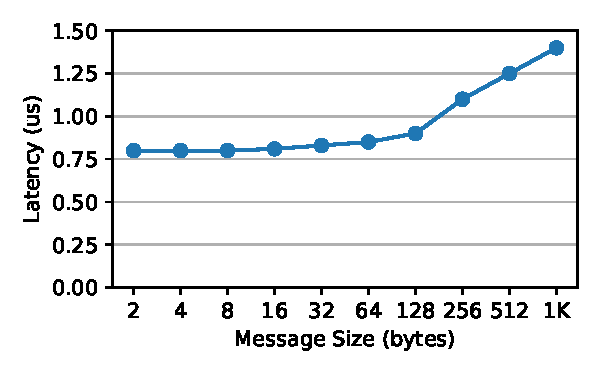
\includegraphics[width=0.99\linewidth]{fig/rdma_latency.pdf}
        \label{fig:rdma_latency}
        % \caption{}
    \end{subfigure}.
    \begin{subfigure}{0.3\linewidth}
        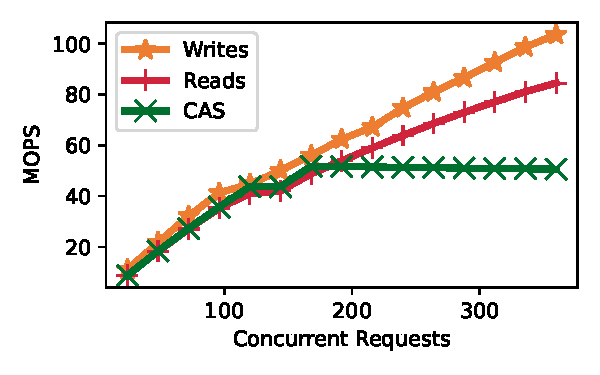
\includegraphics[width=0.99\linewidth]{fig/rdma_concur.pdf}
        % \label{fig:optimistic_failures}
        % \caption{}
    \end{subfigure}
    \begin{subfigure}{0.3\linewidth}
        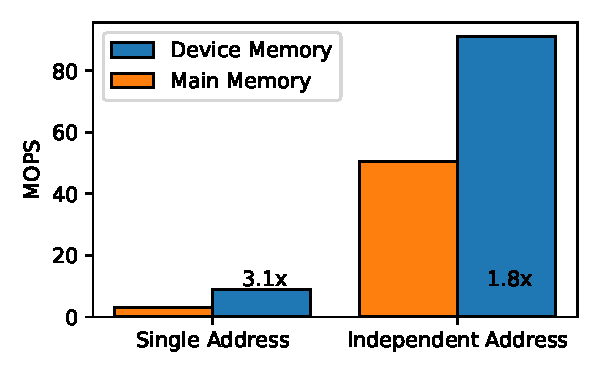
\includegraphics[width=0.99\linewidth]{fig/rdma_cas_throughput.pdf}
        % \label{fig:optimistic_failures}
        % \caption{}
    \end{subfigure}
    \vspace{-1em}
    \caption{
    \textbf{(a)} CX5 RDMA latency vs message size~\cite{rdma-latency}
    \textbf{(b)} RDMA operation scalability
    \textbf{(c)} Compare and swap performance. Device memory vs main memory.
    }
    \label{fig:problems}
\end{figure*}

%concurrent data structures round trips
Concurrent data structure design for remote memory is hard.
Access latency to remote memory is high so round trips per
operation must be minimized to achieve efficiency.
Serialization is particularly hard because there is no
centralized serialization point to guard access to remote
memory. RDMA NIC's provide atomic verbs such as
compare-and-swap (CAS), but these are by no means a silver
bullet.  Each atomic request takes a round trip from client
to server to execute. In the best case lock/unlock requires
two round trips, if multiple locks are required, or locks
are contested the number of round trips increases.

%cpu locking vs rdma
In traditional key value stores (Memcached~\cite{memcached})
the CPU coordinates table access for read, write, and lock
instructions. In contrast RDMA based Key-value
stores~\cite{herd,erpc,pilaf} use a mixture of one-sided (no
cpu) and two-sided (cpu involved) verbs to alleviate the CPU
bottleneck. Reads are typically one sided to bypass the CPU
bottleneck~\cite{pilaf,cell} while writes are typically two
sided so memory-side CPU can orchestrate serialized
operations (e.g. locking) with main memory access latency
(50-100ns).  These small access times keep critical sections
small for CPU based locking, and dramatically increase them
for one-sided RDMA based locking schemes~\cite{clover,
sherman}.

\textbf{Caching:} Modifying a remote data structure requires
clients to have synchronized caches. The cache can either be
accumulated per operation and be discarded or persist across
operations.  Accumulating a cache per operation is slow,
clients must aquire locks, read, then release potentially
many times to complete an operation if the locks are fine
grained. Alternatively clients can persist a cache across
requests in the hope that it will be valid for future
operations.  Clover (a remote memory key value store) caches
pointers to values on clients to enable fast reads when
values are looked up multiple times~\cite{clover}.
Optimistic caching threads a fine line as issuing optimistic
operations which commonly fail may be worse than acquiring
the correct locks.  An ideal caching strategy would enable
clients to succeed in their operations frequently while not
requiring much overhead to maintain. 



%cuckoo hashing optimistic vs locks
\textbf{Critical Sections:} Consider executing an insert
into a concurrent cuckoo hash stored in remote memory. A
client with a cached index may have little or very stale
information about the state of the hash table. To insert the
client must gather information by reading buckets to compute
a cuckoo path. With concurrent clients this leads to a
chicken and egg problem when acquiring locks vs making
reads.

%% optimistic inserts
A client can perform inserts opportunistically by executing
lockless read to learn about the hash table, calculating a
cuckoo path, and executing a sequence of dependent CAS
operations for each step in the path. This approach is
scalable as its critical section is only the length of a CAS
instruction and is only limited by RDMA atomic operation
throughput~\cite{design-guidelines}. However, Paths can
become invalid as other clients running concurrent inserts
invalidate the paths. Figure~\ref{fig:problems}(a) shows the
path insertion failure rate as the number of concurrent
clients grows. This approach minimizes round trips as
dependent CAS operations can be batched thanks to in order
delivery provided by RDMA reliable connections.
Unfortunately failed inserts require additional round trips
to both fix the state of the table, and retry the
insert.\sg{Further - Issuing CAS as a batch leads to complex
path failure cases such a single element in the path failing
while others further down the path succeed. Assesing and
fixing such insertion failures without locks is very hard.}

% lock based inserts
Alternatively to get synchronized information the client can
lock the table, then issue reads. However acquiring locks
without knowledge of the table is hard. A global lock
ensures that all reads are synchronized, but bottlenecks
hash table throughput. Alternatively per bucket locks
enable high throughput but calculating which buckets to lock
requires knowledge of the table. A long cuckoo path may
require locking many buckets and many round trips to gather
information about the hash table.
%%
An ideal protocol would enable clients to perform inserts
without bottlenecks the insert performance of the hash
table, while requiring the fewest round trips to construct
and execute the cuckoo path.

% First, acquiring a lock means a round trip. If the table has
% a single lock, then a client is guaranteed to be able to
% gather all the locks it requires in a single round trip.
% However a single lock does not scale as only a single writer
% can write at a time. This matter is made worse by the fact
% that the critical section of the lock is larger in remote
% memory. Breaking the table up into subtables each with it's
% own lock has it's own problems. An insertion with a long
% path will potentially need to acquire many locks. Each of
% which requires a round trip. Therefore using fine grained
% locking increases the tables scalability but increases it's
% base case insertion time.

\textbf{Read Optimization:} Most data center workloads are
read heavy, therefore read operations should be the most
highly optimized~\cite{datacenter-workloads,facebook-memcached}. Prior
approaches such as RACE require two RDMA round trips per
read. The first is a hash index lookup, the second round
trip reads the actual key-value block. RACE must perform two
round trips because entries in the hash index are limited to
64 bits (CAS width). This is commonly not enough to store
both key and value so RACE can not inline both keys and
values in the index structure. Clover~\cite{clover} enables
single round trips reads. However under contention Clovers
reads require pointer chasing which is known to be expensive
due to each pointer resolution requiring a round
trip~\cite{clio,clover,pointer-chaising}. Ideally we would
be able to ensure that reads complete in a single round
trip.

\textbf{Duplicate Keys:} Clients may issue concurrent
inserts for the same key, given that keys may occupy
multiple location detecting and dealing with duplicate keys
is tricky while maintaining high performance. RACE requires
an extra round trip after each insert to check if a
duplicate key was inserted simultaneously~\cite{race}. An
ideal algorithm would prevent key duplication without
requiring additional overheads.


\section{Design}
\label{sec:design}

\subsection{Locality Hashing}
\begin{figure*}[t]
    \centering
    \begin{subfigure}{0.3\linewidth}
        \begin{align*}
            L_1 &= h_1(k) \\
            L_2 &= L_1 + h_2(k) \% f^{f + log_2(h_3(k))}
        \end{align*}
        % \caption{}
        \label{fig:hash_factor}
    \end{subfigure}
    \begin{subfigure}{0.3\linewidth}
        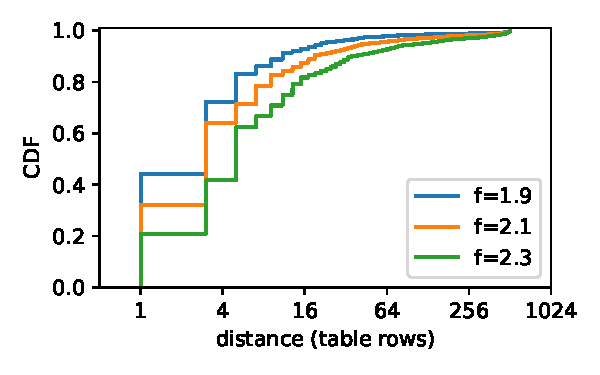
\includegraphics[width=0.99\linewidth]{fig/hash_factor.pdf}
        \label{fig:hash_factor}
        % \caption{}
    \end{subfigure}
    \begin{subfigure}{0.3\linewidth}
        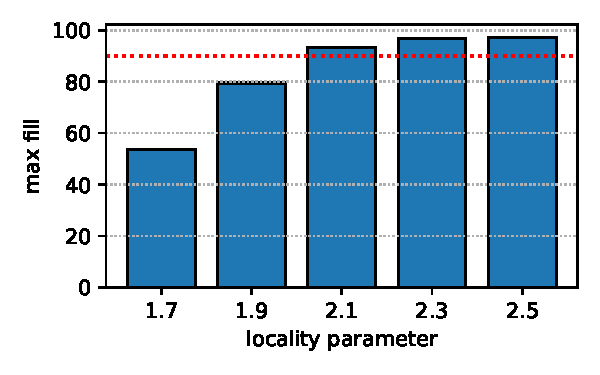
\includegraphics[width=0.99\linewidth]{fig/hash_fill.pdf}
        \label{fig:hash_fill}
        % \caption{}
    \end{subfigure}.
    \vspace{-1em}
    \caption{
    \textbf{(a)} Dependent hashing for factor $f$.
    \textbf{(b)} CDF of distances between cuckoo locations dependent hashing on different exponential factors.
    \textbf{(c)} Exponential factor relation to max fill in cuckoo hash.
    }
    \label{fig:locality-hashing}

\end{figure*}


\begin{figure*}[t]
    \centering
    \begin{subfigure}{0.3\linewidth}
        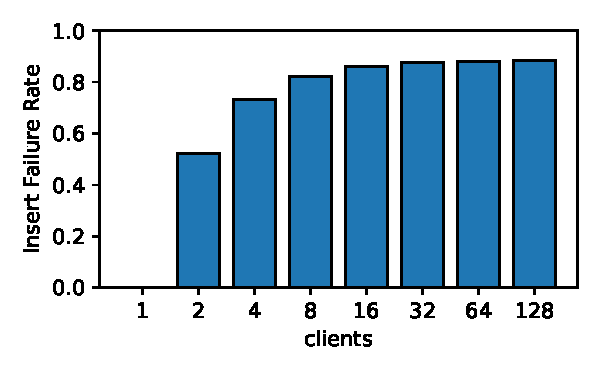
\includegraphics[width=0.99\linewidth]{fig/optimistic_failures.pdf}
        % \label{fig:optimistic_failures}
        % \caption{}
    \end{subfigure}
    \begin{subfigure}{0.3\linewidth}
        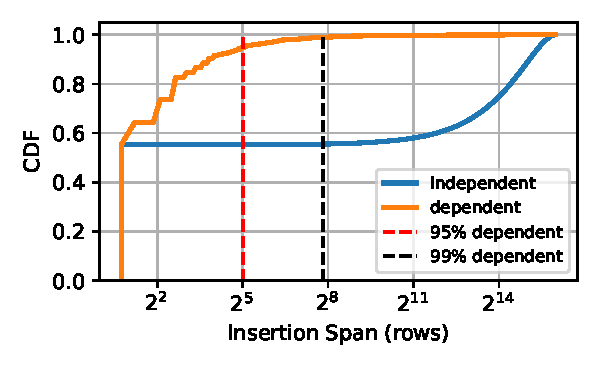
\includegraphics[width=0.99\linewidth]{fig/insertion_span.pdf}
        \label{fig:insertion_span}
        % \caption{}
    \end{subfigure}.
    \begin{subfigure}{0.3\linewidth}
        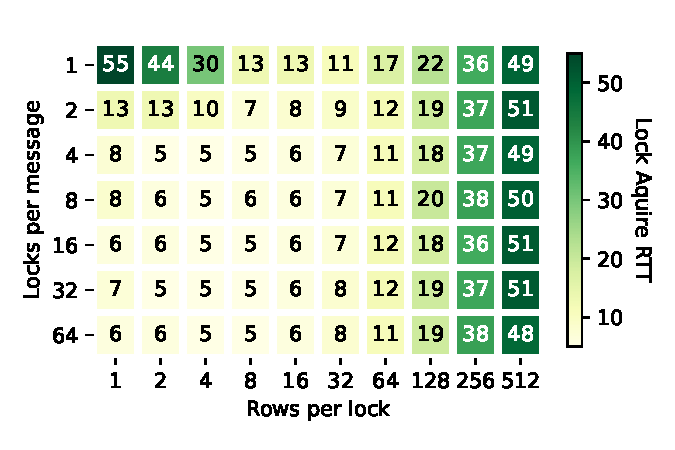
\includegraphics[width=0.99\linewidth]{fig/buckets_per_lock_vs_locks_per_message.pdf}
        \label{fig:tbd}
        % \caption{}
    \end{subfigure}.
    \vspace{-1em}
    \caption{
    \textbf{(a)} Failure rate of optimistic cuckoo insertions.
    \textbf{(b)} CDF of cuckoo spans for dependent and independent hashing. A cuckoo span is the distance between the smallest and largest index in a cuckoo path.
    \textbf{(c)} Round trips (99th percentile) required per insert while filling a table to 100\% while varying the lock per message, and buckets per lock. (\todo{subtract one from each current values include unlocks})
    }
    \label{fig:rdma}

\end{figure*}


Both cuckoo~\cite{cuckoo} and hopscotch~\cite{hopscotch}
hashes are optimized for reads. Cuckoo hashing ensures
constant time reads, while hopscotch hashing ensures that a
read is within a bounded range of it's hash index. Both of
these properties have been noticed by the RDMA key-value
store, and far memory communities for their fast
reads~\cite{memc3,cuckoo-improvements,pilaf,farm}.

Our approach aims to combine the bounded reads of cuckoo
hashing, with the locality properties of hopscotch hashing.
To do so we bound the distance between cuckoo hash
locations. Figure~\ref{fig:rdma}(a) shows the tradeoff
between message size and latency for a ConnectX-5 RDMA NIC.
The latency of small messages (2-128 Bytes) are nearly
identical, and the size of a message must be larger than 1K
before it's latency is 2x that of a small message. Bandwidth
is increasingly available in modern networks with 800Gbps on
the horizon, we tradeoff bandwidth for latency by opting for
larger single messages and fewer round trips. In essence we
make large sloppy reads, and leave it to the client to
reconstruct a result.

Traditional cuckoo hashing calls for two independent hash
functions. We instead make our two hash functions
\textit{dependent}. The first hash function determines the
location a key will be hashed to. The second hash function
determines the maximum distance the second value can have
from the first. A third hash function determines a random
location between the first location, and the bound imposed
by the second. Figure~\ref{fig:locality-hashing}(a) shows
the formula for our dependent hashing function.

A strawman implementation of locality based hashing would
use the first hash function to find a location, and the
second to find a random location within a fixed bound. This
approach quickly leads to failed insertions. Due to the
birthday paradox the probability of a collision is high, and
on large tables the probability that one region of the hash
table will become full, and have not viable path to an open
slot is high. ~\todo{Insert a figure of one of my failed
insertion experiments on a big table}.

Rather than use a static bound we use a dynamic logarithmic
bound with a third hash function. The bound set by the
third hash function is determine by counting the suffix
zeros of the resultant hash and rasing it by an exponential
factor. In the common case the bound is small, but on an
exponentially decrease rate some pairs of values are spaced
far apart. This design enables some pairs to act
as~\textit{waypoints} to other regions of the table. This
method, paired with associative in the cuckoo hash enables
high fill rates while keeping the region of the table any
given key can inhabit small.

The tradeoff between the exponential factor and the mean
distance is fill factor.
Figure~\ref{fig:locality-hashing}(b) illustrates how
increasing the exponential factor shifts the distribution of
distances between cuckoo hash locations.
Figure~\ref{fig:locality-hashing}(c) shows how these same
factors effect the max fill rate of the table before an item
cannot be inserted.


\subsection{Locking}

Traditional wisdom would suggest that because cuckoo hashing
can have long insertion paths it is a poor candidate for
remote memory. Augmenting an insertion path requires making
many modifications to the hash table. There are two
approaches for making path modifications. The first is to
perform a set of compare and swap modification which migrate
an open slot down a path to a location where the new value
is inserted. In this case the client acquires no locks,
however it has no guarantee that it's insertion path with
remain valid as concurrent processes can modify the hash
table with insertions of their own. In this case the client
can opportunistically attempt an insertion path using its
cached information about the table. This strategy has the
potential to fail frequently, and the requires potentially
many reads to be issued for the client to keep it's path
information up to date. ~\todo{insert a plot which shows
path lengths and failure rates from the cukoo approach with
no batching.}

Alternatively a client can aquire locks for the table. Locks
typically have poor performance for disaggregated algorithms
because each lock and unlock operation requires a round
trip. This means that any locking algorithm will have a lock
acquisition phase in which all required locks are collected,
followed by a critical section in which the operations are
executed, and a lock release stage. Using a course grained
locks this approach leads to throughput bottlenecks as it
does not scale with the number of clients. However course
grained locks have the advantage that there are few locks to
aquire, therefore a lock acquisition and release algorithm
takes less round trips. A typical lock acquisition policy
works by acquiring locks in a predefined incremental order to
avoid deadlock. The tradeoff between fine grained and course
locking is clear - fine grained locking allows higher
degrees of parallelism and throughput, while adding higher
latency due to a more complex lock aquire and release stage.
Course locking has lower latency aquire and release, but
limits throughput as many clients will contest the same
locks.

Locality hashing enables very efficient locking due to RDMA
masked CAS
operations~\cite{advanced-transport,scalable-locks}. Without
local hashing fine grained locks would be scattered
throughout the hash table. Locality hashing increases the
probability that an insertion path is within a bounded
region of the hash table.  This means that a lock table with
lock locations corresponding to physical locations in the
hash table will be near one another.  
%%
Figure~\ref{fig:rdma}(b) shows the insert span in buckets
using both dependent and independent hashing on a table with
500K entries and 8 entry buckets. A span is calculated as
the distance between the lowest index and the highest index
in a cuckoo path. Past 50\% independent hashing spans a
random range in the table (whenever a displacement occurs on
insert). With dependent locality based hashing 95\% of
inserts span less than 32 buckets, and 99\% less than 256.
%%
RDMA masked CAS operations allow a client to set a 64 bit
mask along with the new, and old values of the cas
operation. This enables the client to atomically set up to
64 contiguous locks. Using these operations clients can
dramatically decrease the number of round trips required to
acquire locks.
%%
Lock granularity effects performance under contention. Using
values from Figure~\ref{fig:rdma}(b) if locks are per bucket
96\% of lock acquisitions can be completed with a single RTT
masked cas. If locks span 4 buckets 99\% of requests can be
completed in a single round trip.
%%
Figure~\ref{fig:rdma}(c) Shows the tradeoff between lock
granularity and the number of locks which can be set in a
single message with locality hashing turned on. The values
reported are the 99th percentile number of round trips
required to acquire locks up to a 90\% fill factor on a
table with 4096 entries and 8 entries per bucket, and 8
concurrent clients. The biggest factor in round trip times
is the number of locks per bucket. On the far right side of
the heatmap (512) only a single global lock exists. Further
the benefit in terms of locks per message falls off quickly
after 1. RDMA masked CAS are beneficial as they allow for
fine grained locking, but setting 3 or more locks per
message has little effect up to 90\% fill rate.

RDMA atomic throughput is
limited~\cite{design-guidelines}~\todo{[swordbox]}. Reducing
the number of atomic messuages also reduces hardware
limitations on the number of operations. Our lock table is
also small in compairision to the true hash table, each lock
is a single bit, and bits can correspond to multiple rows of
the table if we need to save space~\todo{lock size, vs locks
per message figure}. Because we can save lock space due to
masked cas we can also make use device mapped memory for
faster lock aquisition~\cite{sherman}. RDMA device mapped
memory reduces request latency by executing RDMA operations
onto memory which resides on the RDMA NIC. This memory is
highly constrained~\todo{4MB CX5,CX6}, it removes the need
for a PCIe round trip thereby reducing lock aquisition
latency by aproximatly 2x.

\subsection{Table Design}

We design our table with flexibility in mind. Unlike RACE
which is constrained to 64bit table entries due to CAS width
we can store table entires of arbitrary size as table
updates are made with locks and RDMA writes. We support
inlined values in the index for small keys and values to
support single round trip reads. We support a second format
using extents for variable sized values.
Figure~\ref{fig:table-diagram} illustrates our table design.
Each entry includes an extent bit to indicate if the entry
is inlined or stored in an extent.  We make use of device
mapped memory on recent RDMA NIC's (ConnectX-5+) to reduce
locking latency~\cite{sherman} and enable higher throughput.
Device mapped locking avoids an expensive PCIe round trip,
and reduces on NIC blocking when acquiring locks.


\begin{figure}[t]
    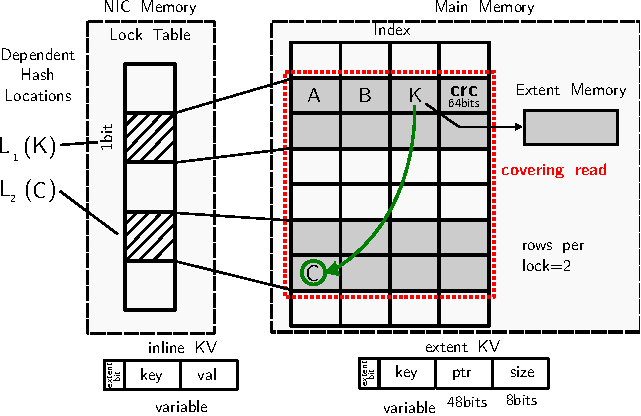
\includegraphics[width=0.99\linewidth]{fig/table-diagram.pdf}
    \caption{Rcuckoo's table design}
    \label{fig:table-diagram}
\end{figure}.


\subsection{Protocol}

\begin{figure}[t]
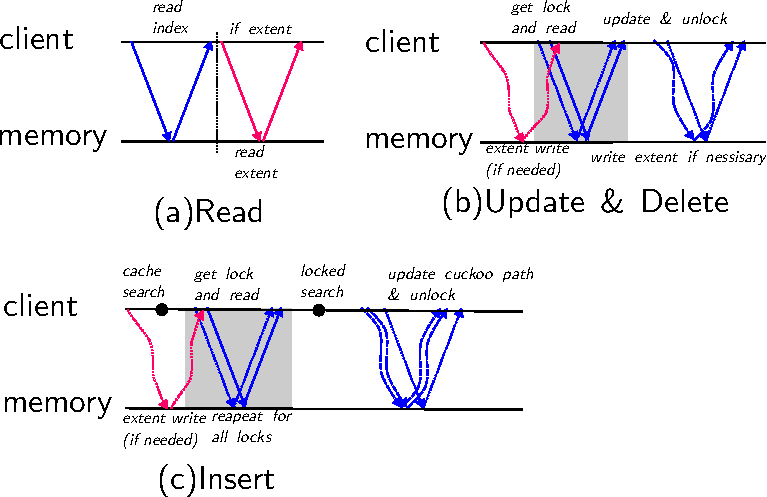
\includegraphics[width=0.99\linewidth]{fig/message_diagram.pdf}

\caption{Rcuckoo's protocol for reads, inserts, deletes and
updates. Blue lines are index accesses, and red lines are
extent accesses. Solid lines are reads, dotted lines are
CAS, and curved dashed lines are writes. }

\label{fig:message_diagram} \end{figure}.

Using locks instead of opportunistic concurrency greatly
reduces the round trips required to perform operations.
Insertions into a cuckoo hash require one message for each
entry in the cuckoo path. Executing the insertion
opportunistically with CAS operations enables concurrent
reads, and insertions, but each swap along the path is
blocking as it requires the prior CAS to complete. The round
trips required to perform an opportunistic search is tied to
the length of the cuckoo path. Further as inserts can run
concurrently path insertions can fail. A single failed
insert along the cuckoo path requires the client to stop and
retry it's insert. Alternatively using locks to guard
buckets can guarantee that cuckoo paths can be executed
without failure. Therefore all cuckoo path swaps can be
batched together into a single round trip.

Clients need their caches to be synchronized with the remote
hash table in order to generate correct cuckoo paths. We
batch reads with RDMA masked CAS operations to synchronize
their caches. When a lock request is issued a single read
which spans the range of the lock request is generated. The
read is issued after the lock request, although the two are
batched together. RDMA reliable connections ensure that on a
single QP operations are executed in order. Therefore if the
lock request returns successfully the batched read will
return synchronized values from the hash table which will
remain unmodified while the lock is held.

Clients with synchronized reads can generated cuckoo paths
which are guaranteed to be valid with lock search.
Therefore, all cuckoo path updates can be issued in a single
batch. Further, CAS operations can be swapped with writes.
Writes have higher throughput than CAS, and slightly lower
latency. We add checksums to our table entries to enable
concurrent reads~\cite{pilaf,cell}.  ~\todo{insert RDMA
benchmark for writes and cas.}

Given this propery our protocol for lock aquisition is as
follows. The client performs a search on its local cache for
an insertion path. A set of locks required for the insert
are generated. The locks are broken into a sequence of RDMA
masked CAS operations. Reads which span the range of each
locked bucket are generated alongside the maksed CAS
operations. Clients issue the lock request and the read
behind it. Once the locks are aquired and the reads are
received the clients cache is up to date.

The insertion path the client used to aquire locks may be
invalid after the lock have been aquired. The client
performs a second search for an insertion path only
searching entries from buckets it has locked. If a path
exists the client generates a sequence of write requests,
and unlock requests. The client issues writes and unlocks in
a batch. This read-lock, search, write-unlock pattern along
with locality hashing ensures that in most cases insertions
(as well as deletes and updates) are performed in two round
trips.

Our protocol saves round trips in comparison to RACE, which
uses three round trips in the common case. On inserts RACE
must re-read the hash table to ensure that concurrent CAS
operations did no insert duplicates. With our algorithm we
can simply check for duplicates by reading both insertion
hash locations when acquiring locks. On updates RACE must
read the index, then the data, and then perform the update
as the index is not large enough to store the key. 

RACE requires that each hash table index is 64 bits so it
can be atomically modified by a CAS. Because we use locks
our index can store larger entries containing the key. It
further enables us to store values in the index enabling
single RTT reads. This strategy increase our common case
read size in excahnge for latency~\todo{evaluation section}.
This same pattern is true in RACE for deletes. 
\todo{insert protocol message figure}

\textbf{Key Duplication:} Unlike RACE our algorithm can
prevent duplicate keys easily on insert. Cuckoo hashing
inserts to exactly one bucket, which is read during the lock
acquisition phase. If a duplicate key is found the client
can abort. If the bucket is full, a duplicate key may exist
in it's alternative bucket. Our clients issue a read to the
inserted keys alternative bucket during lock acquisition. If
the lock returns successfully and no duplicate exists in
either bucket then no duplicates exist as the successful
lock ensures that no other client is currently moving the
key to another location as part of a concurrent insert.


\textbf{Reading:} For inlined reads client complete reads in
a single round trip. We trade off latency for bandwidth by
issuing a single read rather than two for reads which span a
small enough range to fit into a single message. This
increases bandwidth consumption per read, but drops the
overall processing required by the memory NIC. Our reading
threshold is configurable. We chose to read up to 512 bytes
in a single read as this covers over 50\% of all reads for
64 bit table entries~\ref{fig:locality-hashing}.

\subsection{Search}
Cuckoo hashing insert traditionally uses random
replacement~\cite{cuckoo}. Random replacement requires
little computation, however at high fill rates it leads to
long cuckoo paths which require many locks, and reduce
concurrent throughput. BFS search finds the shortest path
and has been demonstrated to increase system throughput with
fine grained locking~\cite{algorithmic-improvements}.

BFS search is computationally intensive. Locality based
hashing enables us to leverage more efficient search
strategies. Because locality hashing increases the
probability that a cuckoo hashing location is close we can
use an informed search algorithm to find open slots close to
bucket a key hashes to. 

In the case of BFS the target bucket is unknown, therefore
all paths must be explored. We use A* search, an algorithm
which takes a goal location, and a distance heuristic as
input. A* is known to find shortest paths in much better
average case times than BFS. A* requires two additional
inputs, a distance heuristic and a goal location.

\textbf{goal location}: Locality hashing increases the
probability that an open slot near the insertion target
location can terminate a cuckoo path. Our algorithm collects
open slots near the original hash location as candidate goal
locations. By default we set the number of candidate goal
locations to 5. Gloal locations are collected by starting at
the $h_1(k)$ location and iterating through the hash
table both forward and backwards through the table one index
at a time. Buckets with open slots are added to the
candidate list until the limit is reached. \todo{I could
improve this search time by tracking the list of open
buckets and using binary search on them.}.

\textbf{Search Heuristic}: A* requires a heuristic for
distance which is a strict underestimate of the true
distance to a goal. A typical heuristic for search is the
euclidean distance between two points. A * guarantees that
if the search heuristic is a strict underestimate of the
true distance to the goal then the path found will be the
shortest path. In our case we use the distance between a
goal state and a current state is unknown as the distance
between any two buckets is the result of our locality
hashing function which has no upper bound. However we can
estimate the distance between two buckets by using the mean
distance of our locality hash function. This approach does
not guarantee that we find the shortest path, however it
does find short paths in the common case, and results in
very short search times.

\section{Implementation} We implement our algorithm in
Python and emulate client based RDMA using a custom built
simulator consisting of 1k lines of python. 

\textbf{Simulator:} Our simulator is event based and does
not emulate network transit time, processing time, or failed
packets. Clients, memory, and switches are modeled as finite
state machines, and the network as FIFO queues. Events are
scheduled randomly, between clients, memory, and the
network. RDMA verbs are modeled as function pointers with
arguments passed by the client.

\textbf{Rcuckoo:} Cuckoo is implemented in 1.2k lines of
python. A* is implemented by hand, with the use of python's
standard heap library for priority queuing. Clients store
complete copies of the remote hash table index locally, and
none of the extent in simulation. In practice for better
resource utilization cached pages of the index could be
released using LRU. Our current implementation does not
include extents, all table accesses are inlined.

\textbf{RACE:} We implement RACE~\cite{race} to the best of
our abilities as no publicly available implementation is
available. We only model the RACE index. In cases where
blocking calls are made to RACE's extent we assume they
succeed and simply reissue a read to the index to model the
round trip incurred by the extent lookup. We model RACE's
blocking behavior exactly in this way. We reached out to
RACE's authors to check our implementation's correctness and
were able to correlate our fill factor results with theirs.

\section{Evaluation}
\label{sec:eval}

\begin{figure*}[ht]
    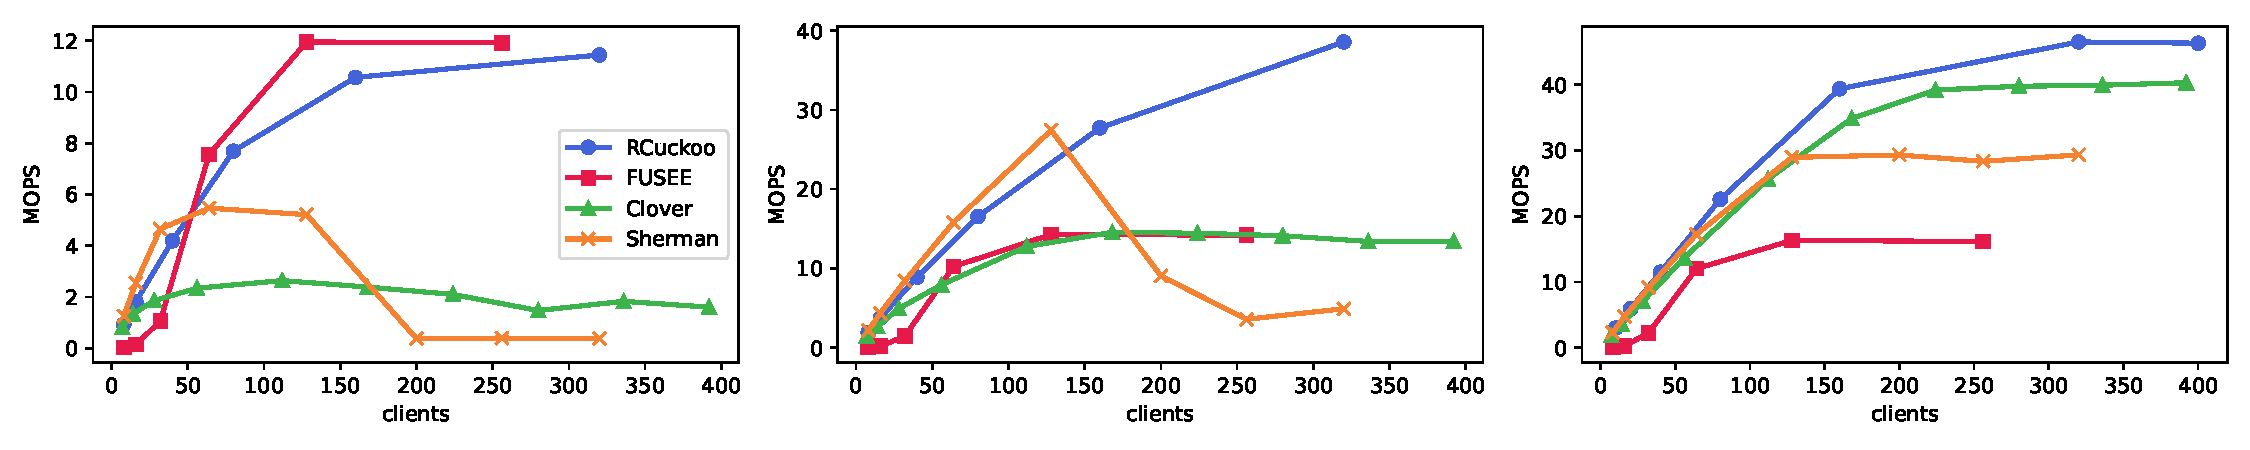
\includegraphics[width=0.99\linewidth]{fig/hero_ycsb_throughput.pdf}
    \caption{race vs rcuckoo simulated throughput}
    \label{fig:ycsb_throughput}
\end{figure*}

\begin{figure*}[ht]
    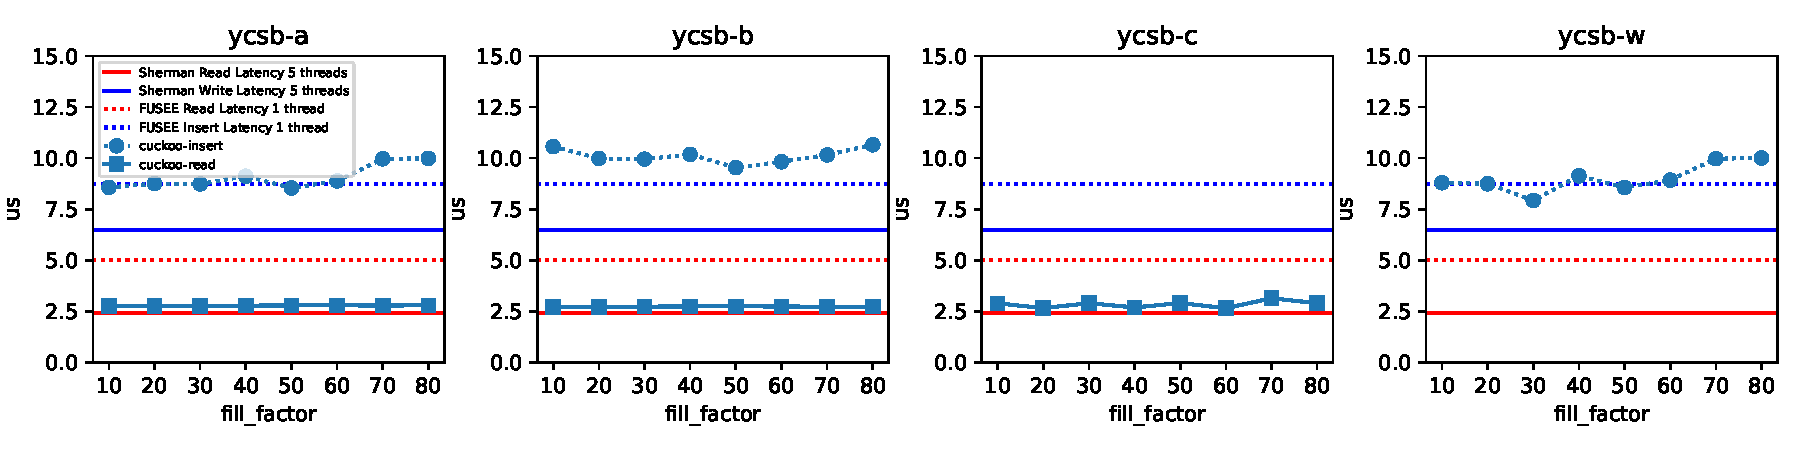
\includegraphics[width=0.99\linewidth]{fig/hero_ycsb_fill_latency.pdf}
    \caption{race vs rcuckoo workload fill latency}
    \label{fig:ycsb_fill_latency}
\end{figure*}

\begin{figure}[ht]
    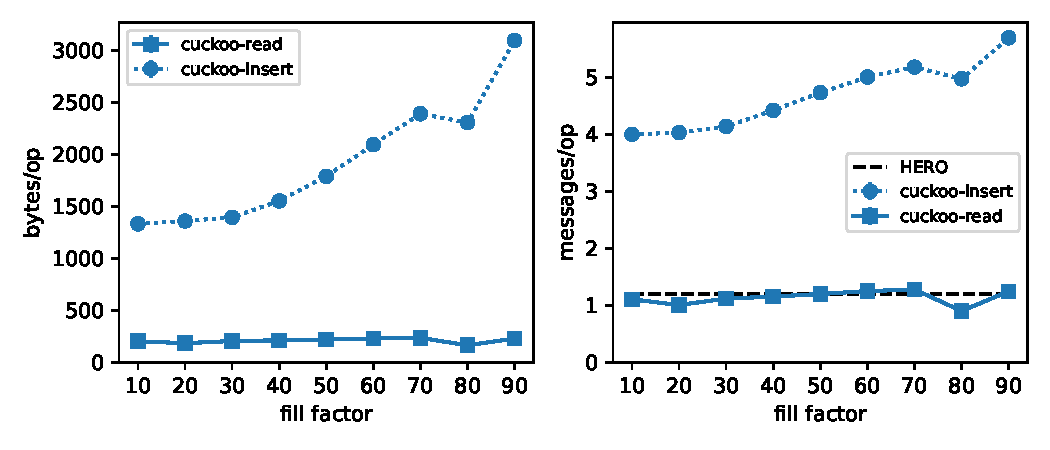
\includegraphics[width=0.99\linewidth]{fig/hero_ycsb_fill_ops_bw.pdf}
    \caption{YCSB-A workload messages and bandwidth per operation as a function of fill factor}
    \label{fig:ycsb_fill_latency}
\end{figure}

\begin{figure}[ht]
    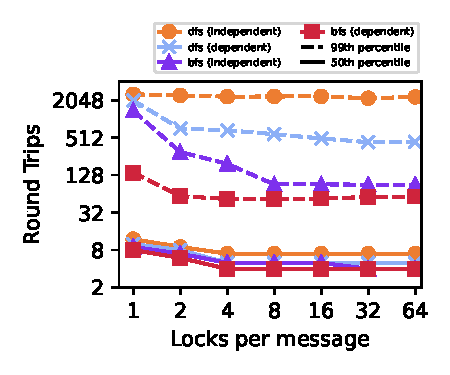
\includegraphics[width=0.99\linewidth]{fig/search_dependence.pdf}

    \caption{Round trips per insert operation compared
    across search functions and hash functions. Dependent
    hash functions with A* have the shortest search times.}

    \label{fig:search_dependence}
\end{figure}

Our evaluation is run entirely in simulation. The goal of
our evaluation is to demonstrate the practicality of Rcuckoo
by showing by proxy that it supports low latency and high
throughput operations. We measure blocking round trip's as a
proxy for latency to measure throughput we normalize the
number of simulation steps each client runs for before
filling the table. Steps do not correlate directly to time,
however the less time a client spends blocking, and the
fewer steps required to complete an operation are a proxy
for real system throughput.

All of our evaluations are carried out on hash tables with
buckets of size 8, and key-value pairs with 32bit keys and
16bit values. On hash tables with 1 million entries.

\subsection{System Breakdown}

Breakdown of insertion performance 

\subsection{System Performance}


Figure~\ref{fig:ycsb_throughput} shows the throughput of race vs rcuckoo for YCSB workloads.

YCSB-A, YCSB-B, and YCSB-C, YCSB-W, for latency.
YCSB-A, YCSB-B, and YCSB-C, YCSB-W, for throughput.
YCSB-A, YCSB-B, and YCSB-C, YCSB-W, for operations per second
YCSB-a, YCSB-b, and YCSB-c, YCSB-w, for bandwidth.



\subsection{Search Performance:}

\textbf{Hashing Algoritms:} Rcuckoo hashing requires
executing many hash compuations. We evalute our A* search
alorithm abolute performacne on various hash functions and
show how this values effect our overall fill factors.

\textbf{A* search vs BFS:} We compare the performance of A*
vs BFS for locally computed insertions. A* performance
directly effects system throughput as this algorithm is run
twice on every insert.


\section{Conclusion}
\label{sec:conclusion}

\section{Challenges}
\label{sec:problems}

High access latency and failures are the root cause of
difficulty in designing a fully disaggregated index. Each
operation must be crafted to minimize the round trips and
ensure the table never reach an unrecoverable state. This
section describes the challenges of designing a lock-based
fully disaggregated cuckoo hash.

\textbf{Synchronization:} Clients must synchronize their
local caches prior to directly modifying a shared table in
remote memory. Cuckoo paths locations are uniformly
distributed so searching for a valid cuckoo path naively
requires iterative random reads to be made throughout the
table. As section~\ref{sec:cuckoo-back} shows the path
constructed by these expensive reads are also quickly
invalidated by contention from other insertions.
Proactively acquiring locks on each read can ensure caches
remain synchronized until a valid cuckoo path is found.
However, acquiring locks one at a time randomly throughout
the table is both expensive and prone to deadlock and course
grain locking (as shown in the following section) quickly
throttles performance as more clients are added. An ideal
synchronization scheme would simultaneously read and lock a
minimal set of table rows in a single round trip. Designing
a solution close to this ideal is a key challenge.

% \textbf{Caching:} Modifying a shared structure from remote
% clients requires cache synchronization. Opportunistic
% updates speculate on the state of the unified cache while
% pessimistic updates acquire locks then read, write, and
% unlock. Porting prior cuckoo hashing algorithms to remote
% memory directly would result in poor performance as clients
% iteratively read one bucket at a time during search and then
% aquire locks~\cite{cuckoo-improvements, memc3, pilaf}.
% Determining how to accumulate a clients cache to perform an
% insert in the fewest number of round trips is a key
% challenge in building a remote cuckoo hash table.

% Accumulating a cache per operation is slow,
% clients must aquire locks, read, then release potentially
% many times to complete an operation if the locks are fine
% grained. Alternatively clients can persist a cache across
% requests in the hope that it will be valid for future
% operations.  Clover (a remote memory key value store) caches
% pointers to values on clients to enable fast reads when
% values are looked up multiple times~\cite{clover}.
% Optimistic caching threads a fine line as issuing optimistic
% operations which commonly fail may be worse than acquiring
% the correct locks.  An ideal caching strategy would enable
% clients to succeed in their operations frequently while not
% requiring much overhead to maintain. 


\textbf{Critical Sections:} Designing a fast, and fine
grained critical section for updates is a main challenge. As
a strawman consider an opportunistic approach to cuckoo
hashing. When a client wants to insert it iteratively reads
the remote index constructing a cuckoo path. Once an open
slot is found it executes a series of CAS operations to
perform the insert. If one element along the path is updated
the entire update will fail.
Figure~\ref{fig:cuckoo-problems}(a) shows the path insertion
failure rate as the number of concurrent clients grows using
this approach on a table with 10k entries filled to 90\%.
The failure rate of operations grows to over 80\% and with each
failure the algorithm must restart.

A naive lock based approach suffers from an inverse problem.
Using a single global lock all updates will succeed however
given a latency of 2us and two round trips to lock and
unlock, the theoretical limit of such an approach is 250k
operations per second, which in practice is much lower. As
such any lock based approach must used fine grained locks.
Figure~\ref{fig:cuckoo-problems}(c) illustrates the extent
of the problem. Using an insertion algorithm described later
in the paper, we measure the round trips per insert for
various lock sizes and locks we can set per message. A
single lock per message requires 55 round trips per insert
at the 99th percentile when each row in the table has an
independent lock. Simultaneously locks protecting large
chunks of the table bottleneck quickly due to lock
contention.  Acquiring multiple locks demands a deadlock
free algorithm in which each atomic acquisition must be
performed in order.  This challenge makes is difficult to
aquire many locks efficiently as acquiring many locks far
apart in memory requires many round trips.

% %cuckoo hashing optimistic vs locks
% \textbf{Critical Sections:} Consider executing an insert
% into a concurrent cuckoo hash stored in remote memory. A
% client with a cached index may have little or very stale
% information about the state of the hash table. To insert the
% client must gather information by reading buckets to compute
% a cuckoo path. With concurrent clients this leads to a
% chicken and egg problem when acquiring locks vs making
% reads.

% %% optimistic inserts
% A client can perform inserts opportunistically by executing
% lockless read to learn about the hash table, calculating a
% cuckoo path, and executing a sequence of dependent CAS
% operations for each step in the path. This approach is
% scalable as its critical section is only the length of a CAS
% instruction and is only limited by RDMA atomic operation
% throughput~\cite{design-guidelines}. However, Paths can
% become invalid as other clients running concurrent inserts
% invalidate the paths. Figure~\ref{fig:cuckoo-problems}(a) shows the
% path insertion failure rate as the number of concurrent
% clients grows. This approach minimizes round trips as
% dependent CAS operations can be batched thanks to in order
% delivery provided by RDMA reliable connections.
% Unfortunately failed inserts require additional round trips
% to both fix the state of the table, and retry the
% insert.\sg{Further - Issuing CAS as a batch leads to complex
% path failure cases such a single element in the path failing
% while others further down the path succeed. Assesing and
% fixing such insertion failures without locks is very hard.}

% % lock based inserts
% Alternatively to get synchronized information the client can
% lock the table, then issue reads. However acquiring locks
% without knowledge of the table is hard. A global lock
% ensures that all reads are synchronized, but bottlenecks
% hash table throughput. Alternatively per-bucket locks
% enable high throughput but calculating which buckets to lock
% requires knowledge of the table. A long cuckoo path may
% require locking many buckets and many round trips to gather
% information about the hash table.
% %%
% An ideal protocol would enable clients to perform inserts
% without impeding insertions in other portions of the hash
% table, while requiring the fewest round trips to construct
% and execute the cuckoo path.

% First, acquiring a lock means a round trip. If the table has
% a single lock, then a client is guaranteed to be able to
% gather all the locks it requires in a single round trip.
% However a single lock does not scale as only a single writer
% can write at a time. This matter is made worse by the fact
% that the critical section of the lock is larger in remote
% memory. Breaking the table up into subtables each with it's
% own lock has it's own problems. An insertion with a long
% path will potentially need to acquire many locks. Each of
% which requires a round trip. Therefore using fine grained
% locking increases the tables scalability but increases it's
% base case insertion time.

\textbf{Read Optimization:} Most data center key-value
workloads are read heavy, therefore read operations should
be the most highly
optimized~\cite{datacenter-workloads,facebook-memcached}.
Ideally we would be able to ensure that reads complete in a
single round trip.

Prior optimistic approaches require two round trips or more
per read, because RDMA CAS operations are only 64 bits. Most
key-value indexes are organized as both an index and an
extent, where the index contains 64 bit entries which can be
atomically modified. The extent contains both the key, and
the value and it pointed to by the index. This is not ideal
for small key value pairs which could be embedded in the
index for fast reads if the atomic width were larger. Some
approaches enable single round trips for repeat reads as the
location of the extent can be cached, however they do not
enable single round trip reads from clients without up to
date caches.~\cite{clover}.

% Prior approaches such as RACE require
% two RDMA round trips per read. The first is a hash index
% lookup, the second round trip reads the actual key-value
% block. RACE must perform two round trips because entries in
% the hash index are limited to 64 bits (CAS width). This is
% commonly not enough to store both key and value so RACE can
% not inline both keys and values in the index structure.
% Clover~\cite{clover} enables single round trips reads.
% However under contention Clovers reads require pointer
% chasing which is known to be expensive due to each pointer
% resolution requiring a round
% trip~\cite{clio,clover,pointer-chaising}. 


\textbf{Duplicate Keys:} Clients may issue concurrent
inserts for the same key, given that keys may occupy
multiple location detecting duplicate keys can require
additional checks. RACE and FUSEE require an extra round
trip after each insert to check if a duplicate key was
inserted simultaneously~\cite{race,fusee}.  An ideal
algorithm would prevent key duplication without requiring
additional overheads.
\section{Design}

In this section we describe our design for a fully
disaggregated lock-based cuckoo hash. First we describe a
new dependent hashing algorithm which increases the
probability that two cuckoo hash locations will be near one
another. We design a new locality aware locking scheme,
designed to minimize network round trips.

\todo{syncronize with the rest of the section}



% Next
% we describe a locality aware search algorithm (A*) which
% produces short insertion paths in the cuckoo hash. Finally
% we outline a protocol for insert, read, update and delete to
% the cuckoo hash which uses our locking and search schemes.

\label{sec:design}

\begin{figure*}[t]
    \centering
    \begin{subfigure}{0.3\linewidth}
        \begin{align*}
            L_1 &= h_1(k) \\
            L_2 &= L_1 + (h_2(k)\mod f^{f + log_2(h_3(k))})
        \end{align*}
        % \caption{}
        % \label{fig:hash_factor}
    \end{subfigure}
    \begin{subfigure}{0.3\linewidth}
        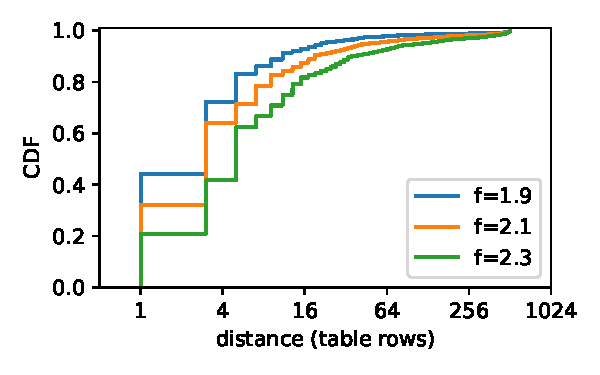
\includegraphics[width=0.99\linewidth]{fig/hash_factor.pdf}
        % \label{fig:hash_factor}
        % \caption{}
    \end{subfigure}
    \begin{subfigure}{0.3\linewidth}
        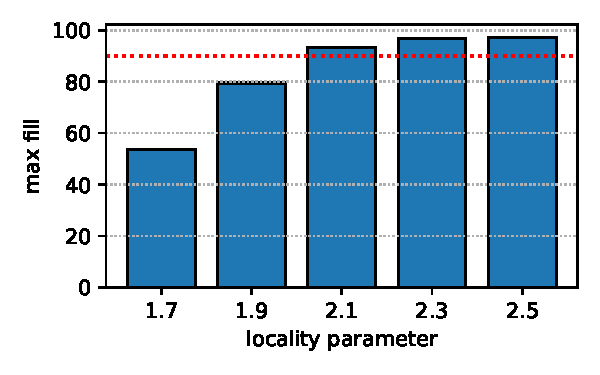
\includegraphics[width=0.99\linewidth]{fig/hash_fill.pdf}
        % \label{fig:hash_fill}
        % \caption{}
    \end{subfigure}.
    \vspace{-1em}
    \caption{
    \textbf{(a)} Dependent hashing for factor $f$.
    \textbf{(b)} CDF of distances between cuckoo locations dependent hashing on different exponential factors.
    \textbf{(c)} Exponential factor relation to max fill in cuckoo hash. 90\% fill marked in red.
    }
    \label{fig:locality-hashing}

\end{figure*}




\subsection{Dependent Hashing}

Cuckoo and hopscotch hashes are optimized for
reads~\cite{cuckoo,hopscotch} and have been used extensively
in RDMA key value
stores~\cite{memc3,cuckoo-improvements,pilaf,farm}. Both
hashes are read optimized, cuckoo hashing ensures at most
two reads are required (both can be done in parallel), while
hopscotch hashing ensures the locality of a read to a
specific location.

Our approach aims to combine the constant time reads of
cuckoo hashing with the locality properties of hopscotch
hashing. Traditional cuckoo hashing requires two independent
hash functions which set key locations uniformly at random.
We use two ~\textit{dependent} hash functions to increase
locality between key locations. The first hash function
selects a row in the cuckoo table uniformly at random. The
second second hash function selects a location randomly from
the following $n$ rows after the first hash location. The
value of $n$ is not constant. A third hash function $h_3(x)$
generates values of $n$ according to an exponential
distribution. We use a constant factor $f$ to control the
exponential function.  Figure~\ref{fig:locality-hashing}(a)
shows the formula for our dependent hash functions.

The constant value $f$ determines the distribution of
distances between key locations.
Figure~\ref{fig:locality-hashing}(b) is a CDF of distances
between key locations for 3 values of $f$. A distance of 1
means that a keys second location is in the row immediately
after it's first location. In the case of $f$=2.3 20\% of
keys have a distance of 1 bucket. Small values of $f$ have
high locality. However, locality is not free. Independent%%
hash functions enable cuckoo hashes to read high fill rates (95\% and higher).
%%
Removing independence increase the probability of
hotspots which cause insert operations to fail. A cuckoo
insertion fails if no sequence of swaps exists which can
produce a valid cuckoo path. Failed insertions require the
table to be resized and directly effect memory utilization.
Therefore $f$ is directly related to the maximum fill factor
a table can achieve using dependent hashing.

% An over
% filled region of the table can quickly lead to deadlocks
% when inserting requiring the table to be resized. $f$ is
% directly related to the max fill factor of the table. Larger
% $f$ values increase the max fill factor, while decreasing
% locality.  

Figure~\ref{fig:locality-hashing}(c) shows the relationship
between $f$ and a tables maximum fill. These values were
generated by inserting into a cuckoo table with 100M entries
until an insertion failed. Table associativity directly
effects fill rate. The higher the degree of associativity
the more likely a valid path will exist. The table used in
Figure~\ref{fig:locality-hashing} has an associativity of 8
similar to prior cuckoo
hashes~\cite{memc3,cuckoo-improvements,pilaf}.


% The associativity of the
% cuckoo hash plays a key role in enabling high fill. The
% higher the degree of associativity the greater degrees of
% freedom search is given to escape local hotspots.

%The second hash function determines the maximum
%distance the second value can have from the first. A third
%hash function determines a random location between the first
%location, and the bound imposed by the second.
% Figure~\ref{fig:locality-hashing}(a) shows the formula for our hashing
% function process, which implements the probabilistic region-size
% selection with a third hash function---akin to the way Bitcoin
% computes its difficulty.
% \textbf{Why not make the second hash function a true expoential?}

% A strawman implementation of locality based hashing would
% use the first hash function to find a location, and the
% second to find a random location within a fixed bound. This
% approach quickly leads to failed insertions. Due to the
% birthday paradox the probability of a collision is high, and
% on large tables the probability that one region of the hash
% table will become full, and have not viable path to an open
% slot is high. ~\sg{Perhaps this justifies a figure, please
% advise.}.

% We use a dynamic exponential bound rather than a static one.
% The dynamic bound is set by raising a constant factor $f$ by
% an exponent determined by a third hash function. Using the
% third hash on the key we count the number of suffix zeros
% and raise the constant factor by itself plus the zero count.
% This distribution generates exponential distances between
% hash locations at exponentially less frequency and is
% tunable with the single parameter $f$.
% %%
% In the common case the bound is small. Exponentially few key
% are spaced far apart and act as~\textit{waypoints} to other
% regions of the table when constructing cuckoo paths. This
% method, paired with bucket associativity enables high fill
% rates while keeping the region of the table any given key
% can inhabit small.

% There is a tradeoff between locality and fill factor.
% Figure~\ref{fig:locality-hashing}(b) illustrates how
% increasing the exponential factor shifts the distribution of
% distances between cuckoo hash locations.
% Figure~\ref{fig:locality-hashing}(c) shows how these same
% factors effect the max fill rate of the table before an item
% cannot be inserted. As will be shown in the following
% sections read, and insert performance improve with better
% locality. Therefore fill factor and performance can be
% traded off directly by changing the exponential factor. In
% our evaluation we found an exponential factor of 2.3 to give
% the best results in terms of end to end performance and
% bandwidth consumption.


\subsection{Locking}

\begin{figure*}[t]
    \centering
    \begin{subfigure}{0.3\linewidth}
        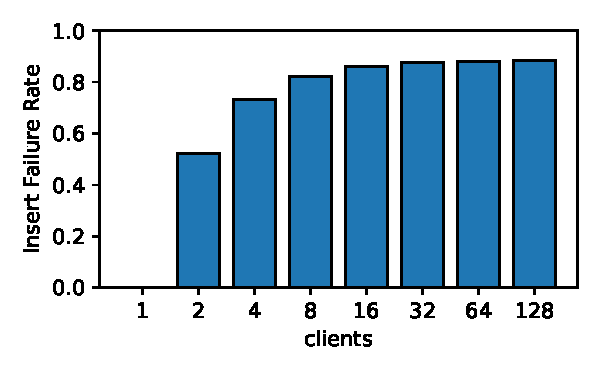
\includegraphics[width=0.99\linewidth]{fig/optimistic_failures.pdf}
        % \label{fig:optimistic_failures}
        % \caption{}
    \end{subfigure}
    \begin{subfigure}{0.3\linewidth}
        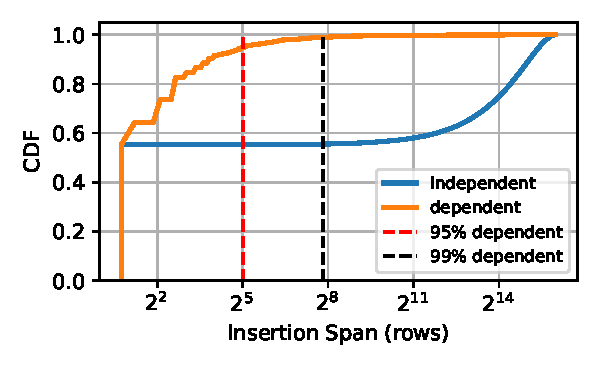
\includegraphics[width=0.99\linewidth]{fig/insertion_span.pdf}
        \label{fig:insertion_span}
        % \caption{}
    \end{subfigure}.
    \begin{subfigure}{0.3\linewidth}
        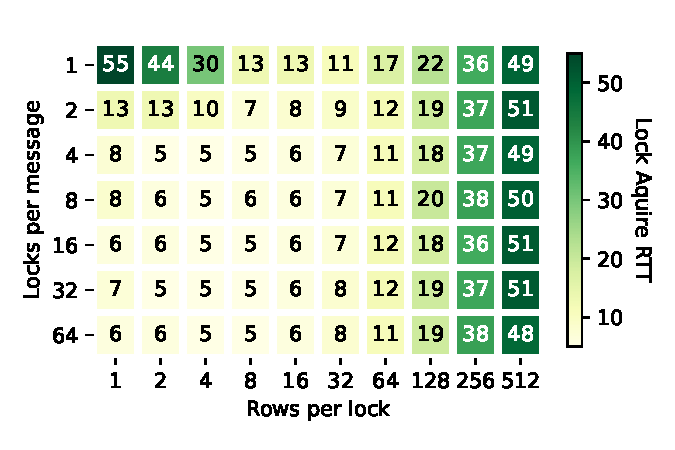
\includegraphics[width=0.99\linewidth]{fig/buckets_per_lock_vs_locks_per_message.pdf}
        \label{fig:tbd}
        % \caption{}
    \end{subfigure}.
    \vspace{-1em}
    \caption{
    \textbf{(a)} Failure rate of optimistic cuckoo insertions.
    \textbf{(b)} CDF of cuckoo spans for dependent and independent hashing. A cuckoo span is the distance between the smallest and largest index in a cuckoo path.
    \textbf{(c)} Round trips (99th percentile) required per insert while filling a table to 100\% while varying the lock per message, and buckets per lock. \todo{subtract one from each current values include unlocks}
    }
    \label{fig:cuckoo-problems}

\end{figure*}

Rcuckoo uses locks rather than optimistic operations
(compare-and-swap) so table entries can be larger than 64
bits. This enables fast reads, as both keys, and values can
reside directly in the table index. Locking can be
expensive, as a naive deadlock free aquire and release
protocol can incur many round trips.  in this section we
describe our lock table, and locking protocol designed to
achieve fast locking in an average of two round trips.

Our lock table is an array of contiguous bits where each bit
is a lock, and each lock guards one or more sequential
buckets. The size of the lock table in bytes equals the
number of hash table rows, divided by the number of rows
each lock guards (rows per lock). The size of a lock table
for a cuckoo table with 100M entries, 8 entries per row, and
16 rows per lock is 102KB.  Lock table size, and rows per
lock are important variables as they enable us to utilize
two features of modern RDMA NICs, mainly device mapped
memory, and masked compare and
swap~\cite{rdma-masked-cas,sherman}.

Device mapped memory is a small reigon of on NIC memory,
typically on the order of 256KB. This memory executes
one-sided RDMA operations faster than host memory as the
operations need not make a PCIe round trip. This memory is
especially performant for atomic operations as the NIC would
otherwise have to queue dependent atomic request to host
memory. Figure~\ref{fig:rdma-benchmarks}(c) shows the
performance boost from device over host memory for atomic
operations.

The second NIC feature we exploit is masked compare and swap
operations ~\ref{fig:rdma-masked-cas}. Masked cas operations
enable clients to set individual bits rather than 64 bit
spans. As our lock table is tightly packed this enables
clients to aquire locks without any additional knowledge
about the lock table as would be required for unmasked cas.

Together with locality hashing these features enable the
following fast locking protocol. When a client requires
locks it calculates all lock indexes locally. Lock indexes
are the row the client must lock divided by the number of
rows per lock. Once the set of locks is calculated the
client breaks the set of locks into separate locking
requests. If the locks are within 64 entries of each other
all locks are packed into a single masked compare and swap
packet. If the span of locks is greater than 64 a second
packet is generated with all locks in the next range of 64
packed together into a single packet. To avoid deadlocks
lock request are issued one at a time. Clients repeatedly
request the same locks until they are acquired. Lock
releases are done in a single batch.

% We use RDMA device memory for our lock
% table~\cite{rdma-masked-cas}. To aquire locks clients
% locally determine which locks they require for their
% operation, and then issue RDMA masked CAS operations to the
% device memory. This approach enable clients to aquire up to
% 64 contiguous locks with a single RDMA operation and enable
% clients to aquire locks without synchronizing the state of
% the lock table prior to acquisition (non masked CAS would
% need the state of all locks prior to issuing the request.).

This locking scheme in conjunction with dependent hashing
enables most client operations to aquire locks in a singe
round trip. Update and insert operations require at most two
locks, one for each key location. Using $f$ of 2.3 90\% of
key pairs are within 64 rows of each other so even with row
per lock 90\% of updates and deletes can be completed in two
round trips. In practice we use 16 rows per lock which
results in 99.7\% of updates and deletes resulting in two
round trips.

Inserts can span arbitrary regions of the table and are a
harder case than updates and deletes.
Figure~\ref{fig:cuckoo-problems}(b) shows the span in rows
of cuckoo paths for a table with 100K rows. These spans are
the difference between the highest and lowest row locked
during insertion. Using dependent hashing 95\% of insertions
span 32 rows or less, and 99\% of insertions span 256 rows
or less. Using 16 rows per lock each masked cas can cover
1024 rows of the table ensuring that 99.5\% of insertion
locks can be acquired in a single round trip.

% Using this locking scheme locality hashing greatly improves
% locking performance. With independent hashing the locks for
% a cuckoo path are scattered randomly throughout the table.
% Therefore, a round trip is required for each lock, and each
% lock must be acquired in order to avoid deadlock. With
% locality, and the ability to lock up to 64 sequential locks
% most insertions can be performed with a single round trip
% for locking. In both cases lock release can be batched in a
% single round trip.

% Figure~\ref{fig:cuckoo-problems}(b) shows the insert span in
% buckets using both dependent and independent hashing on a
% table with 500K entries and an associativity of 8. A span is
% calculated as the distance between the lowest index and the
% highest index in a cuckoo path. Past 50\% independent
% hashing spans a random range in the table (whenever a
% displacement occurs on insert). With dependent locality
% based hashing 95\% of inserts span less than 32 buckets, and
% 99\% less than 256.


% Traditional wisdom would suggest that because cuckoo hashing
% can have long insertion paths it is a poor candidate for
% remote memory. Both opportunistic, and lock based approaches
% have significant drawbacks.
% %%
% As an example consider an opportunistic approach in which
% many clients are inserting concurrently to a table. Clients
% making inserts first make reads of the table to locally
% calculate a cuckoo path for their insertion. After the reads
% complete the client constructs a cuckoo path and starting
% from the open slot issues dependent CAS requests migrating
% the open slot backwards to the insertion bucket.
% %%
% Figure~\ref{fig:cuckoo-problems}(a) shows the failure rate
% of this insertion scheme as a factor of clients running
% inserts on a table with 500K entries with a bucket
% associativity 8. Cuckoo paths calculated from client caches
% quickly become invalid as the number of clients grows.
% %%
% Alternatively deadlock free lock acquisition requires more
% round trips and has larger critical sections. Each lock must
% be acquired in order with a dependent CAS request which
% incurs an additional round trip per lock. Using course
% grained locks reduces the number of acquisitions but
% throttles throughput as concurrent insertions are more
% likely to contend shared locks.

% Locality hashing increases the probability that an insertion
% path is within a small region of the hash table which in
% turn increases the probability that fine grained locks will
% be near one another. 
% %%
% Figure~\ref{fig:cuckoo-problems}(b) shows the insert span in
% buckets using both dependent and independent hashing on a
% table with 500K entries and an associativity of 8. A span is
% calculated as the distance between the lowest index and the
% highest index in a cuckoo path. Past 50\% independent
% hashing spans a random range in the table (whenever a
% displacement occurs on insert). With dependent locality
% based hashing 95\% of inserts span less than 32 buckets, and
% 99\% less than 256.
% %%
% RDMA masked CAS operations allow a client to set a 64 bit
% mask along with the new, and old values of the cas
% operation. So locks can be acquired with minimal knowledge
% of the remote lock table. This enables the client to
% atomically set up to 64 contiguous locks independently which
% dramatically reduces the round trips required to aquire
% locks.

% Lock granularity effects performance under contention. Using
% values from Figure~\ref{fig:cuckoo-problems}(b) if locks are
% per bucket 96\% of lock acquisitions can be completed with a
% single RTT masked cas. If locks span 4 buckets 99\% of
% requests can be completed in a single round trip.

% Increasing the number of buckets each lock guards can reduce
% the number of locks required for an operation.
% Figure~\ref{fig:ycsb_fill_latency}(c) shows the tradeoff
% between lock granularity and the number of locks which can
% be set in a single message with locality hashing turned on.
% The table has 512 rows total to illustrate the effect of a
% single global lock.

% The values
% reported are the 99th percentile number of round trips
% required to acquire locks up to a 90\% fill factor on a
% table with 4096 entries and 8 entries per bucket, and 8
% concurrent clients. The biggest factor in round trip times
% is the number of locks per bucket. On the far right side of
% the heatmap (512) only a single global lock exists. Further
% the benefit in terms of locks per message falls off quickly
% after two. RDMA-masked CAS are beneficial as they allow for
% fine-grained locking, but setting 3 or more locks per
% message has little effect up to 90\% fill rate. Reducing
% atomic operations in turn reduces the effect of the RDMA
% atomic bottleneck.  \textbf{Hard to see 3; the figure only shows 2 or 4.}

% Our lock table is small in comparison to the true hash
% table. At its most fine-grained each lock corresponds to
% one bucket (8 entries). Each lock is 1 bit, a lock table for
% a 100 million entry hash table is ~160KB, with a lock
% granularity of 4 buckets this drops to 40KB. This tight
% layout enables us to use device-mapped memory to hold our
% lock table~\cite{design-guidelines,sherman}.
% %We make use of
% Device-mapped memory on recent RDMA NIC's (ConnectX-5+) avoids an
% expensive PCIe round trip, reducing lock acquisition latency.
% This enables up
% to 3$\times$ better throughput on contested locks (see
% Figure~\ref{fig:rdma-benchmarks}(c)), and reduces latency
% for locking.

\subsection{Table Design}

\sg{@alex I've left the proposed table design in}

We design our hash table for fast reads as most data center
key-value workload are read heavy~\cite{facebook-workloads}.
Prior disaggregated indexes such as
~\cite{clover,race,fusee} require two round trips minimum
for first time reads as their indexes do not support
inlining. In the case of RACE and FUSEE index entries are
fixed to 64 bits to support RDMA CAS width operations. This
fact prevents both projects from inlining key value data and
requires them to make a second round trip to an extent to
retrieve data, and check if a key is present in the table.

In our table users can specify the size of their index entries at
initialization time. Key value pairs which are small enough
to fit within the index are inlined, otherwise they are
stored in an extent. Figure~\ref{fig:table-diagram}
illustrates our table design. Each entry includes an extent
bit to indicate if the entry is inlined or stored in an
extent.

\subsubsection{Client Caching}

\todo{expand} Clients cache duplicates of the remote index
to improve the performance of operations. In the case of
insertions clients search their locally cached indexes to
determine a cuckoo path prior to acquiring locks. 

\subsubsection{Memory Allocation}

Prior work has focused on different memory allocation and
hash table resizing schemes. Sherman~\cite{sherman} uses an
allocated thread located on the memory node,
Fusee~\cite{fusee} uses a two tired memory allocation in
which large blocks of memory are allocated on the memory
nodes and fine grained allocation is performed on the
clients. Clover~\cite{clover} statically partitions memory
into large client regions prior to execution and hash
clients entirely manage the space themselves. Network based
allocators such as MIND and Clio~\cite{mind,clio} have
demonstrated the feasibility of high performance
disaggregated allocators, while some have called for
allocators to be built into RDMA~\cite{prism}. We allocate
memory using the same scheme as Clover, as it is simple to
implement and adds no additional overhead. We view memory
allocation as a hard orthogonal problem to the design of
disaggregated indexes and have designed our system
acrostically to the allocator.




\begin{figure}[t]
    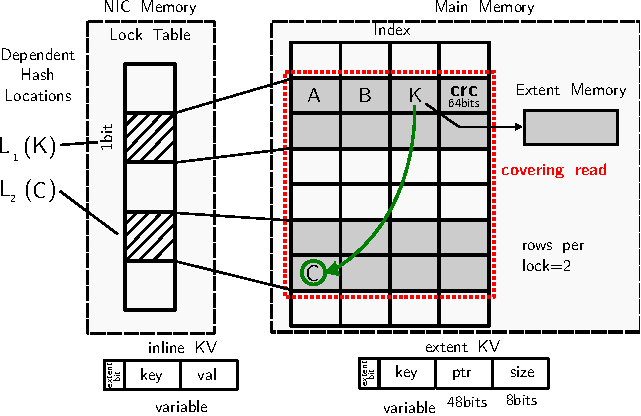
\includegraphics[width=0.99\linewidth]{fig/table-diagram.pdf}
    \caption{Rcuckoo's table design ~\todo{remove extents for this submission}}
    \label{fig:table-diagram}
\end{figure}


\subsection{Protocol}

\begin{figure}[t]
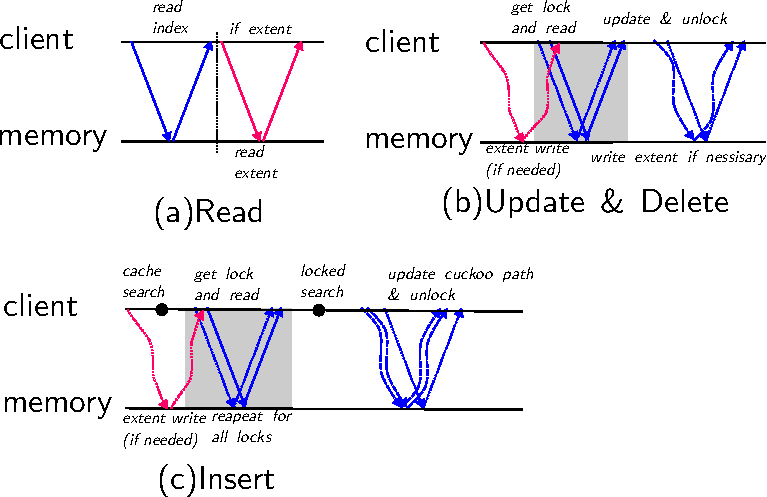
\includegraphics[width=0.99\linewidth]{fig/message_diagram.pdf}

\caption{Rcuckoo's protocol for reads, inserts, deletes and
updates. Blue lines are index accesses, and red lines are
extent accesses. Solid lines are reads, dotted lines are
CAS, and curved dashed lines are writes.}

\label{fig:message_diagram}
\end{figure}

In this section we describe our protocol for reading,
inserting, and performing updates and deletes to an rcuckoo
hash table. Figure~\ref{fig:message_diagram} visualizes our
protocol.

\subsubsection{Reading} 
\label{sec:reading}

Client read request are closely similar to traditional
cuckoo hashing with two additional performance
optimizations. To read a key $k$ clients first locate both
key locations. In default cuckoo hashing two reads are
issued in parallel to both rows. We take advantage of
dependent hashing locality and issue a single read which
captures both rows if the distance between key locations is
less than a predefined threshold. If key locations are in
adjacent rows a single read saves packet processing time,
network bandwidth due to header size, and waiting time as
the client need not wait for a second read to return. Larger
reads consume additional bandwidth but still provide some
additional performance (see Section~\ref{sec:read-threshold}).

If key-value entries are inlined reads complete in a single
round trip. Larger key stored in extents require a second
round trip as clients must first read the index, resolve the
virtual address of the extent and then perform the extent
read.
%%
~\footnote{This design requires exactly one pointer
resolution in expectation that future RDMA NICs may provide
pointer resolution reads as a primitive~\cite{prism}}
%%
As reads are lockless they can occur simultaneously with
writes updating the table. Each entry contains a CRC which
is checked on reads to validate that all writes have
completed~\cite{pilaf,cell}.
%%
We define a read threshold of 512 bytes for our clients.
Approximately 60\% of keys for 64-bit entries with a bucket
size of 8 (see Figure~\ref{fig:locality-hashing}(b)) fall
into this category. This has the advantage of updating the
client cache for future operations.
%, and reduces the header processing required by the NIC.
To reduce bandwidth the size of the threshold can be tuned
down, or turned off with no harm to correctness.

% \subsubsection{Locking and unlocking}

% Update, delete and insertion operations all require locks to
% modify the index. Locks are acquired in incremental order
% from smallest to largest to avoid deadlocks. First the list
% of locks required for the operation is calculated. For
% updates and deletes two locks may be required. Inserts may
% required many locks. The client calculates which locks it
% requires and breaks the list into masked CAS operations
% spanning 64 locks and then issued the requests polling for a
% successful response before moving to the next lock.

% To synchronize the client cache with remote memory we issue
% a \textit{covering read}. A covering read is an RDMA read
% which spans the range of buckets from the lowest lock in the
% masked CAS to the highest. The covering read is issued after
% the masked CAS and ensures the client receives synchronized
% data for the locked buckets while not consuming an
% additional round trip.

% Clients need their caches synchronized with remote memory
% prior to modifying it with writes. We batch reads with lock
% requests to synchronize client caches. RDMA in-order
% delivery ensures that reads issued after a lock request will
% be up to date, as no other client can concurrently modify
% the locked index.  A spanning read is issued for each lock
% request. The read covers each bucket the client locks.  For example, if a
% masked CAS has three locks, reads are calculated for each
% bucket being locked. If the locks cover a range less than
% the read threshold a single read is issued which spans all
% buckets between the locks.  Spanning reads are issued concurrently with
% lock requests.
%Subsequent lock requests are issued prior to
%blocking on reads.

% After locks are acquired the client can execute its critical
% section. Unlock requests are the inverse masked CAS operations of the
% lock requests. Clients issue their critical sections as a sequence of
% (asynchronous) writes followed immediately by unlock operations. RDMA
% in-order delivery ensures that the unlock operations are performed
% after the writes.

\subsubsection{Updates and Deletes}

Updates and deletes are similar operations as both require
two locks. In the locking phase clients calculate and aquire
both locks~\ref{sec:locking}. Updates to inlined entries
issue a single entry sized update directly to the index.
Updates to extents issue three messages first the new extent
is written, the index is updated, and finally the old extend
is set to invalid and marked for garbage collection. In both
cases unlock messages are batched with the update. Similarly
deletes lock both table entries. On deletes clients compact
the row so open entries are always located at the end of the
row~\footnote{Ensuring open entries are at the ends of rows
improves search times for open buckets.}. Extent entries are
marked as invalid in the same round trip. Both updates and
deletes commonly execute in 2 round trips. 3 round trips are
required only if both locks are too far apart to be set in a
single masked cas operation.

\subsubsection{Insert}

Unlike updates and deletes, inserts may require modifying
locations spread across remote memory and require many
locks. The main challenge in performing an insert is
determining which locks to aquire. A naive approach would
use a global lock, or incrementally aquire locks during
search. These approaches are known to throttle throughput,
and require many round trips to
complete~\cite{cuckoo-improvements}. Unlike prior work,
issuing reads to the remote index while searching is
untenable as it will frequently require many round trips to
build a cuckoo path.

We design a novel two stage search approach to minimize
round trips while producing valid cuckoo paths with high
probability.

\textbf{Speculative Local Search:} The first stage of
insertions is a speculative local search. Clients calculate
an cuckoo path by searching their unsynchronized local
caches. While This may not produce a valid cuckoo path it
constructs a speculative cuckoo path which is localized to
the region of the table likely to contain a vaild path. When
the table hash low fill, the speculative path is frequently
correct. Using the speculative path, the client calculates
the locks required for the speculative insertion aquire the
unessisary locks.

Clients synchronize their caches during lock acquisition.
Using the speculative path, clients use a \textit{covering
read} which spans the locked rows. As covering reads can be
large we limit them to the same size as the read threshold.
Covering reads are batched together with lock requests but
are sequenced after. As such the values returned by the read
after a successful lock aquire are fully synchronized.

\textbf{Second Search:} The speculative path may not be
valid after clients have acquired locks and synchronized
their caches. If the speculative path is not valid clients
perform a second search restricted to the rows locked by the
client. Due to dependent hashing cuckoo paths are highly
localized. If locks cover 8 or more rows clients have a high
probability of constructing a valid cuckoo path using the
rows locked by their first search. If clients can not find a
valid path with their second search the client releases it's
locks and tries again. Subsequent searches have a high
likely hood of success as clients retain their caches across
requests. We measure the success rate of second searches in
response to the number of rows per lock in our evaluation
section~\ref{sec:second-search}.

Cuckoo paths and updates are issued in a single batch. If a
valid search path is found path updates are made as a batch
of sequential writes. Unlock operation are batched after the
writes. Writes to the extent precede updates to the table.

% Clients must first aquire
% remote locks and then synchronize their cache before they
% can calculate a guaranteed valid cuckoo path. Acquiring many
% locks speculatively can decrease throughput by blocking
% concurrent clients. Simultaneously performing huge
% synchronizing reads can absorb unessisary bandwidth.


% Determining which locks to aquire is hard as clients
% may have stale caches and many options for potential
% insertions paths.  We use a speculative two-phase search
% strategy to find and execute insertions with high
% probability in two rounds trips. First the client searches
% it's local cache for a potential cuckoo path. Once a path is
% found the client calculates the set of locks it requires and
% attempts to aquire the locks for the speculative cuckoo
% path. As locks are speculative reads synchronize the client
% cache.

% After the speculative locks are acquired the client performs
% a second search only using the locked buckets in the table.
% If no such path can be found, the client releases the locks
% and tries again. If a new path can be found using the locked
% buckets that path is executed and the lock is released.
% This search strategy benefits greatly from course grained
% locks. We have found in practice that setting each lock to
% cover 8 buckets yields the highest performance. Given the
% distribution of the locality hash function there is high
% probability that an insertion path can be found within the
% 64 locked buckets. In the common case this means that
% inserts take only two round trips. On failures the client
% maintains the cache it built during the first search to
% improve its chances of finding a path on the next attempt.


% We use a two-phase search
% strategy to find insertion paths. First the client
% constructs a potential cuckoo path using its cached index.
% The client then attempts to acquire the locks necessary for
% its cuckoo path. Thanks to the spanning reads, once a client
% succeeds in acquring the necessary locks its cache has been
% fully synchronized with the relevant portions of remote
% memory. A second search is then performed using only the
% buckets the client succeeded in locking---which may be the
% same if the client's cache was completely up to date. If
% this search is successful the client calculates the updates
% to the cuckoo path batches them as a series of writes and
% issues them along with it's unlock requests.

% If the first search fails the client performs a read and
% tries again. If this fails the table must be resized. The
% second search may fail because the clients cache was stale
% and the list of locked buckets was insufficient to perform
% the insert. In this case the client releases the locks and
% performs the insertion from the start again by performing an
% unrestricted search on its local cache. In the common case
% insertions take two round trips: We find that when the table is less
% than 50\% full the probability that a cuckoo path has
% length greater than one is low. If extents are
% used the client batches the extent write during its locking
% phase.

% \textbf{Key Duplication:} Unlike RACE our algorithm can
% prevent duplicate keys easily on insert~\cite{race}. RACE
% requires three round trips for inserts, the third re-reads
% the index to ensure no duplicates were inserted
% concurrently.  Alternatively Cuckoo hashing inserts to
% exactly one bucket, which is read during the lock
% acquisition phase. If a duplicate key is found the client
% can abort. If the bucket is full, a duplicate key may exist
% in itts alternative bucket. Our clients issue a read to the
% inserted keys alternative bucket during lock acquisition. If
% the lock returns successfully and no duplicate exists in
% either bucket then no duplicates exist as the successful
% lock ensures that no other client is currently moving the
% key to another location as part of a concurrent insert.


\subsubsection{Search Algorithm} 

Cuckoo paths are highly influenced by the search algorithm 
used to find them. Prior work has used DFS to construct 
cuckoo paths~\cite{pilaf,memc3}. We follow prior work and 
use BFS as it produces the shortest 
paths~\cite{cuckoo-improvements}. Short paths reduce the 
number of locks required. Dependent hashing opens new 
opportunities for search optimization as open slots are more
likely to be close to an initial hash location. As part of
our work we investigated using guided search A* to construct
short paths using locality information. We found that A*'s
performance only improves on BFS at fill rates about 95\%
which are rarely found in practice due to max fill rate
limitations.

% Locality based hashing provides us opportunities for better
% search than traditional cuckoo hashing. Cuckoo hashing
% insert traditionally uses random replacement~\cite{cuckoo}.
% Random replacement requires little computation, however at
% high fill rates it leads to long cuckoo paths which require
% many locks, and reduce concurrent throughput. BFS search
% finds the shortest path and has been demonstrated to
% increase system throughput with fine-grained
% locking~\cite{cuckoo-improvements}.  BFS is computationally
% intensive. Locality based hashing enables us to leverage
% more efficient search strategies. Because locality hashing
% increases the probability that a cuckoo hashing location is
% close we can use an informed search algorithm to find open
% slots close to bucket a key hashes to. 
% %%
% In the case of BFS the target bucket is unknown, therefore
% all paths must be explored. We use A* search, an algorithm
% which takes a goal location, and a distance heuristic as
% input. A* is known to find shortest paths in much better
% average-case times than BFS~\cite{}. A* requires two
% additional inputs, a distance heuristic and a goal location.

% \textbf{Goal location}: Locality hashing increases the
% probability that an open slot near the insertion target
% location can terminate a cuckoo path. Our algorithm collects
% open slots near the original hash location as candidate goal
% locations. By default we set the number of candidate goal
% locations to 5. Goal locations are collected by starting at
% the $h_1(k)$ location and iterating through the hash
% table both forward and backwards through the table one index
% at a time. Buckets with open slots are added to the
% candidate list until the limit is reached. 

% \todo{I could
% improve this search time by tracking the list of open
% buckets and using binary search on them.}.

% \textbf{Search Heuristic}: A* requires a heuristic for
% distance which is a strict underestimate of the true
% distance to a goal. A typical heuristic for search is the
% euclidean distance between two points. A * guarantees that
% if the search heuristic is a strict underestimate of the
% true distance to the goal then the path found will be the
% shortest path. In our case we use the distance between a
% goal state and a current state is unknown as the distance
% between any two buckets is the result of our locality
% hashing function which has no upper bound. However we can
% estimate the distance between two buckets by using the mean
% distance of our locality hash function. This approach does
% not guarantee that we find the shortest path, however it
% does find short paths in the common case, and results in
% very short search times.

\subsection{Replication, and scalability} 

\todo{no real replication probabily delete, consider moving
to future work / limiations} At the time of writing RCuckoo
does not support replication although replication is in no
way a complication for our existing algorithms. On inserts
clients aquire locks from a master memory node as described
in section~\ref{sec:insert}, after locks are acquired on the
master node updates, deletes, or cuckoo paths are broadcast
to replicas. Replication requires a clients to wait for
responses from replicas before issuing unlock messages as
the client can not rely on RDMA RC connection in order
delivery across the multiple replica connections.

\todo{We don't span multiple memory nodes} When using
multiple memory machines each machine is initialized with an
equal portion of the cuckoo index and lock table. Clients
calculate which machine to issue their requests to when
generating requests.


\section{Evaluation}
\label{sec:eval}

We evaluate RCuckoo by directly comparing its performance in terms of
throughput and latency against representative state-of-the-art
disaggregated key/value stores.  When accessing large values,
aggregate throughput is limited by link rate, so we focus on small
key/value pairs where the table management overhead is most
significant.  When values are small enough to be stored inline,
RCuckoo outperforms existing systems while delivering competitive
insert latencies.  Using fault injection, we show that our distributed
approach to client failure detection and recovery enables RCuckoo to
sustain high throughput even though 100s of clients are failing per
second.  Finally, we justify our design decisions through a series of
micro-benchmarks. Specifically, we quantify the benefit RCuckoo
extracts from its locality enhancement and speculative search strategy
before measuring the impact of
%conduct sensitivity analysis
%of our choice of locality parameter,
%covering read threshold, and
index-table entry size.

\subsection{Implementation}

We have built two separate versions of RCuckoo, an 8.7~K-line C++
implementation tuned for high performance and a 12~K-line Python
implementation that simulates RDMA operations to facilitate
correctness testing. Both implementations will be made available on
GitHub at the time of publication.  We report results using our C++
implementation which requires OFED-4.9 to support masked CAS
operations and device-mapped memory on ConnectX-5 NICs.  At the time
of writing extent entries and delete operations are supported by our
Python implementation alone; the experiments consider reads, inserts
and updates of inlined table entries.


\begin{figure*}[ht]
  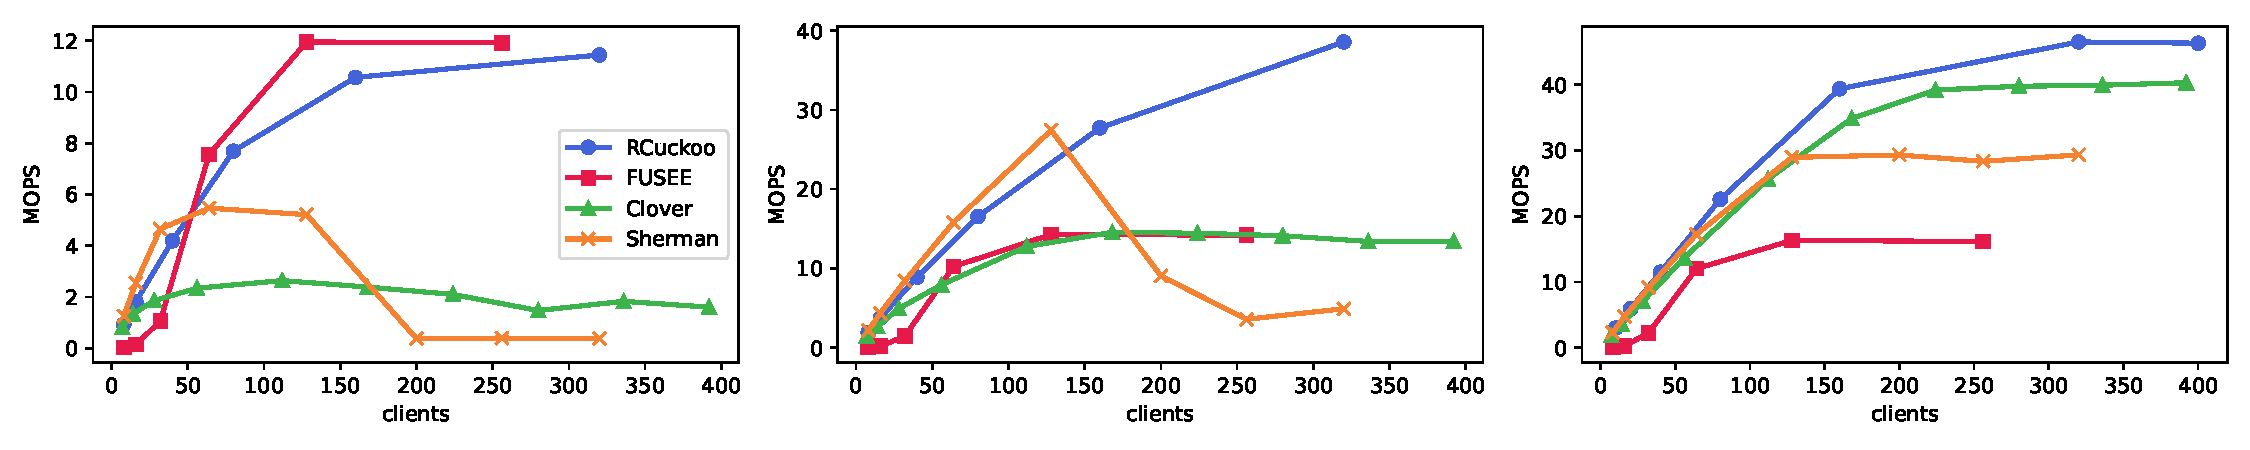
\includegraphics[width=0.99\linewidth]{fig/hero_ycsb_throughput.pdf}
  \vskip -1em
\caption{Throughput as a function of the number of clients for three different workloads (Zipf $\theta$=0.99): \textbf{(a)} Read only (YCSB-C), \textbf{(b)} YCSB-B 95\% read, 5\% update and \textbf{(c)}
    50\% read 50\% update (YCSB-A).}
\label{fig:ycsb_throughput}
\vskip -1em
 \end{figure*}


\subsection{Testbed}

We conduct our evaluation on an 9-node cluster of dual-socket Intel
machines. Each CPU is an Intel Xeon E5-2650 clocked at
2.20~GHz. Each machine has 256~GB of RAM with 128~GB per NUMA
node. All machines have a single dual-socket ConnectX-5 attached to a
100-Gbps Mellanox Onyx switch. In our RCuckoo experiments we use one
sever as the memory server and the rest a client machines
spreading threads evenly across machines.

%\subsection{Comparison systems}

We compare RCuckoo against three recent RDMA key/value stores with
different designs, FUSEE~\cite{fusee}, Clover~\cite{clover}, and
Sherman~\cite{sherman}.  While none have the exact same assumptions or
feature set as RCuckoo, each represents an apt comparison point for
different aspects.  To avoid biasing our evaluation, we consider the same
workloads (YCSB) as the authors of the previous systems.
%
%We directly compare RCuckoo against three disaggregated
%key-value stores  Each system has distinct design
%tradeoffs. 
%%
%%
%%

\textbf{FUSEE} is a fully disaggregated key/value store that
represents the closest available comparison point to RCuckoo.  While
both employ only 1-sided RDMA operations, FUSEE eschews locking in
favor of optimistic insertions.  FUSEE clients use CAS operations
to manage fixed, 64-bit index table entries that contain pointers to
values stored in extents.  Due to its reliance on CAS operations, FUSEE is unable to support inlined storage of small
values like RCuckoo, forcing all reads to require two round trips.
%Fusee is the closest comparison we have to illustrate
%the tradeoffs between locks and optimistic concurrency.
%is a key-value store designed for full
%disaggregation~\cite{fusee}.  It is built on top of RACE~\cite{race}
Unlike RCuckoo, FUSEE is designed to support replication.  To remove the overhead of replication, 
%While RACE represents a more direct comparison to RCuckoo, no open
%source implementation of RACE is available.  Instead,
we deploy FUSEE with a single memory node.
%FUSEE/RACE hashing uses fixed-sized 64-bit index entries
%to in order to employ RDMA compare-and-swap operations for updates. As
%such, RACE-based systems cannot store key-value pairs in the index
%table itself and require a second round trip even for reads of small values.
%on reads to recover
%extent entries which contain full key value pairs.

\textbf{Clover} is only partially disaggregated---it requires a
metadata server to manage its index structure---but can deliver higher
read performance than FUSEE on read-only workloads.  Clover is
designed to leverage remote persistent memory and implements both
reads and updates using one-sided RDMA operations.  Moreover, unlike
FUSEE---and similar to RCuckoo---Clover reads are self verifying.
%Clover uses index caching to optimize reads.  When re-reading key-value
%entries clover can as it directly
%reads the entry without negotiating with the index.
In contrast to prior comparisons~\cite{fusee} that force
clients to consult the metadata server on each read, we allow Clover
to take advantage of its client caching to achieve maximum performance
on read-heavy workloads.

%% Clover is a partially disaggregated system which uses
%% two-sided RDMA operations to modify the index and one-sided
%% operations for updates, deletes, and reads.

%% Sherman a disaggregated B-Tree and the only system at the
%% time of writing which uses locks and not optimistic
%% concurrency to guard its index. Our performance comparison
%% with Sherman is not apples to apples. Sherman maintains
%% ordered key-value pairs for range queries and thus has
%% higher overheads on updates than the other systems.

\textbf{Sherman} is the highest-throughput distributed key/value
storage system of which we are aware that employs locks.  Sherman
maintains a B-tree that spans multiple servers and supports range
queries, a feature none of the other systems---RCuckoo
included---provide.
%is a B-tree designed for remote memory~\cite{sherman}.
%and high write
%throughput.
%Unlike Clover and FUSEE which employ optimistic consistency control,
%Sherman uses locks to guard updates similar to RCuckoo.
On the other
hand, Sherman clusters are not fully disaggregated: each node in a
cluster is a peer with many CPU cores and a single memory core
that is responsible for servicing allocation RPC calls from clients.
%Unlike the other systems
%Sherman is cluster based, and does not support a having
%isolated memory machines.
%All machines are equal nodes in a
%cluster and run both a memory controller and client threads.
As such, Sherman does not encounter the same bandwidth bottlenecks as
the other systems because requests are partitioned across all
machines in the cluster.
%However, it assumes that collocated clients can resolve lock
%contention locally and clients collocated with their segment
%of the B-Tree can perform local operations. These
%assumptions enable Sherman to have high performance under
%contention even though it uses locks and manages a more
%complex data structure than the unordered key-value stores.
%While Sherman does not meet the fully disaggregated model it
%does provide a good comparison for RCuckoo as it is the only
%other system to use locks in remote memory.


% \subsubsection{Clover}
% \todo{insert a short clover description}

\begin{figure*}[ht]
    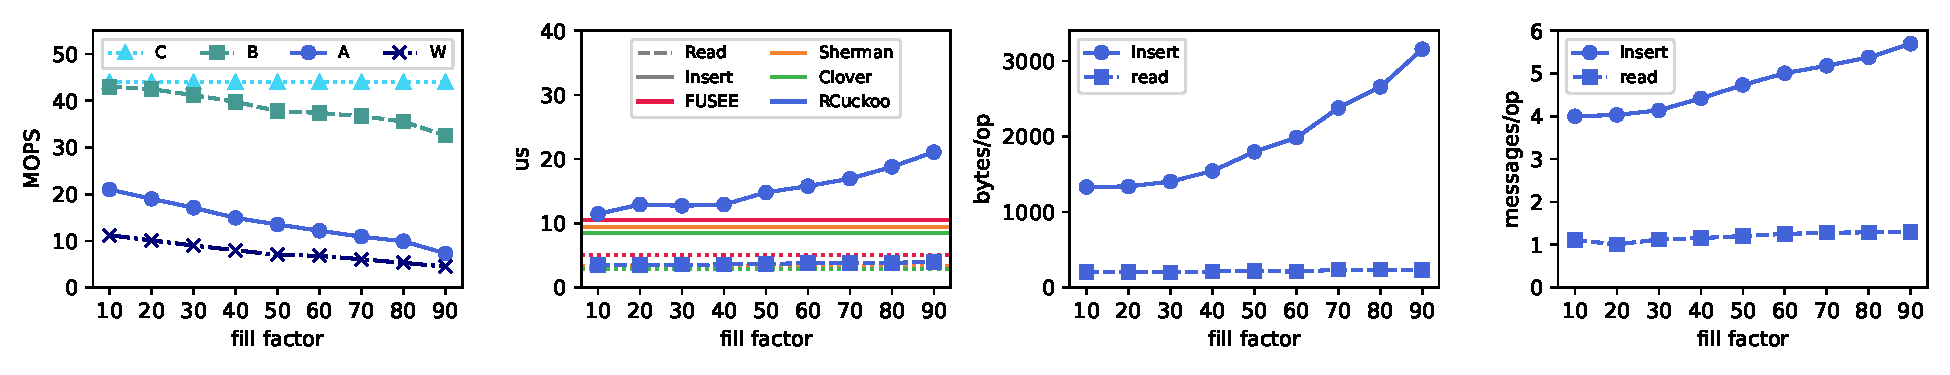
\includegraphics[width=0.99\linewidth]{fig/hero_ycsb_fill.pdf}
\vskip -1em
    \caption{Performance as a
    function of fill factor. \textbf{(a)} Throughput for four different YCSB insert workloads, \textbf{(b)}
    median operation latency, \textbf{(c)} mean operation size, and \textbf{(d)}
    mean RDMA message count per operation under YCSB-A.}
\vskip -1em
    \label{fig:ycsb_fill}
\end{figure*}

% \begin{figure}[ht]
%     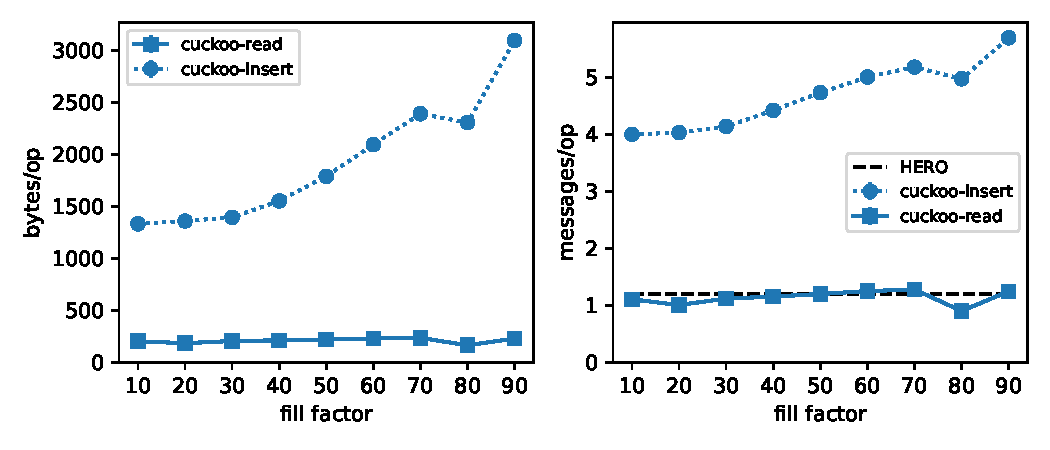
\includegraphics[width=0.99\linewidth]{fig/hero_ycsb_fill_ops_bw.pdf}
%     \caption{YCSB-A workload messages and bandwidth per operation as a function of fill factor}
%     \label{fig:ycsb_fill_ops_bw}
% \end{figure}



\subsection{Performance}

We start by considering throughput and latency on the classical YCSB
workloads which employ varying mixes of read and update operations
before turning to the more complex insert operation.  RCuckoo delivers
the highest performance on reads and updates across all settings,
while insert performance varies as a function of table fill factor.
Even in the worst case, however, RCuckoo limits I/O amplification to
around 2$\times$.
\todo{What is the row/read size?  How close are we
  to line rate?}

\textbf{Throughput.} Figure~\ref{fig:ycsb_throughput} shows throughput
in terms of operations per second for RCuckoo, FUSEE, Clover, and
Sherman on three different YCSB workloads.  Moving from left to right,
the left-most graph is read-only (YCSB-C), the middle graph is 95\%
read and 5\% update (YCSB-B), and the right-most graph presents a 50\%
read, 50\% update mix (YCSB-A).  For each system, we provision a
100-M-entry table and prepopulate it with 90~M entries that each
consist of a 32-bit key and 32-bit value (we consider larger sizes in Section~\ref{ss:mb}).  We plot the aggregate throughput of a variable number of
clients concurrently accessing entries according to a Zipf(0.99)
distribution.

In a read-only (YCSB-C) workload, FUSEE suffers from its extent-based
value storage.  RCuckoo, Clover, and Sherman perform similarly at
low-to-moderate levels of concurrency, but they separate at scale.
Sherman's read algorithm is more complex than RCuckoo's leading to
lower top-end performance.  Clover's client-side caching shines under
this skewed workload, where almost all reads hit in a client's index
cache, requiring only a single read for the value; its performance
degrades under a more uniform workload (not shown).  RCuckoo, on the
other hand, reads inlined values in a single round trip
regardless of the distribution, leading to the highest performance.

Absolute performance for all systems decreases with increasing update
rate due to contention.  Even with only 5\% updates (YCSB-B), the
picture changes dramatically.  Sherman performs well at low levels of
concurrency due to its single-round-trip-reads, but hits a severe
bottleneck due to lock contention on the skewed access pattern.  (Sherman performance is
improves---but does not surpass RCuckoo---for uniform workloads, not
shown, where lock contention is less of an issue.)
Caching is less effective with updates, bringing Clover's throughput in line with FUSEE.
%performs similarly to FUSEE on YCSB-B; we
%suspect that with tuning Clover's read-only performance could be
%brought to par with RCuckoo.
%, and is the
%most competitive with RCuckoo in read-only scenario.  When it is able
%to leverage its client index cache,

On the 50/50-mixed YCSB-A workload RCuckoo and FUSEE perform
similarly, although we are unable to scale FUSEE past 250 clients in
our testbed while RCuckoo continues to scale.
%begins to surpass FUSEE after about 125 clients.  FUSEE's maximum performance is gated by its requirement for an additional round trip per operation (to
%retrieve the extent).
Sherman begins to suffer from lock contention even earlier, topping
out around 5 MOPS before collapsing.  Clover performs worst under
write-heavy workloads due to its inability to effectively leverage
caching with a constantly changing index structure.

%On read-mostly (YCSB-B) and read-only (YCSB-C) workloads RCuckoo
%pulls ahead.
%, extracts even further benefit from its ability to complete
%reads in a single round trip by collapsing most reads into a single
%RDMA request (Section~\ref{sec:read_threshold}).
%  While lock contention is not an issue in the read-only YCSB-C,

% \begin{figure*}[t]
%     \centering
%     \begin{subfigure}{0.24\linewidth}
%       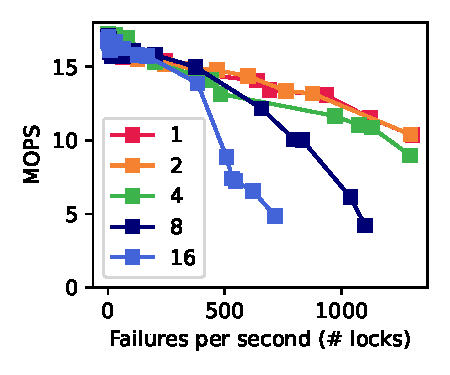
\includegraphics[width=0.99\linewidth]{fig/fault-rate.pdf}
%           \end{subfigure}
%     \begin{subfigure}{0.24\linewidth}
%         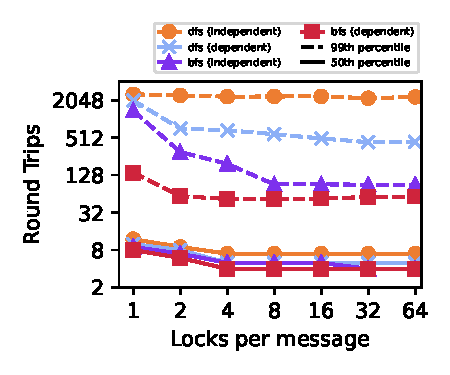
\includegraphics[width=0.99\linewidth]{fig/search_dependence.pdf}
%         % \label{fig:hash_fill}
%         % \caption{}
%     \end{subfigure}
%     \begin{subfigure}{0.24\linewidth}
%         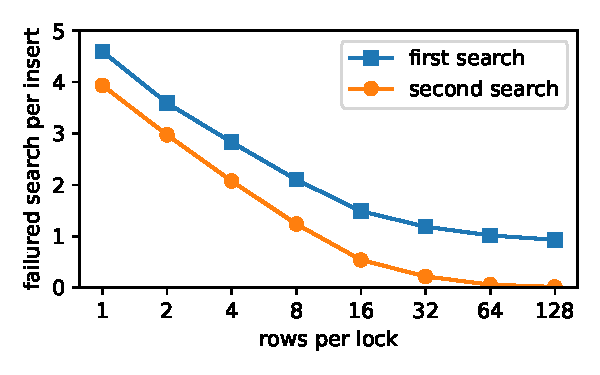
\includegraphics[width=0.99\linewidth]{fig/search_success_lock_size.pdf}
%         % \label{fig:hash_factor}
%         % \caption{}
%     \end{subfigure}
%     %\begin{figure}[ht]
%     \begin{subfigure}{0.24\linewidth}
%       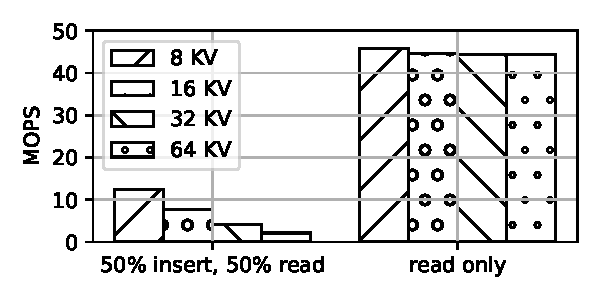
\includegraphics[width=0.99\linewidth]{fig/entry_size.pdf}
%           \end{subfigure}
% \vskip -1em
%     \caption{RCuckoo microbenchmarks:
%       \textbf{(a)} YCSB-A throughput vs. client failure rate,
%           \textbf{(b)} round trip times required to acquire locks on insert,
%     \textbf{(c)} insert second-search success rate as a function of lock granularity, and
%     \textbf{(d)} throughput vs. key/value-entry size for YCSB-A (insert) and YCSB-C (read-only) workloads.
%     }
%     % \label{fig:microbenchmarks}
%              \label{fig:microbenchmarks}
% \vskip -1em
% \end{figure*}


\begin{figure}
\centering
      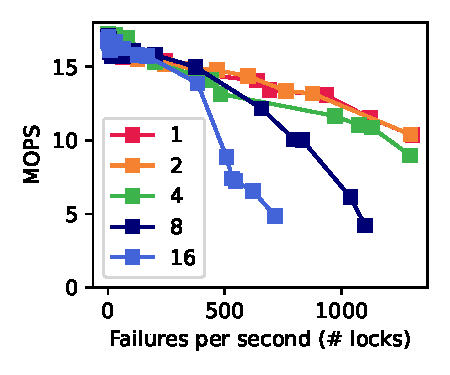
\includegraphics[width=0.99\linewidth]{fig/fault-rate.pdf}
\caption{YCSB-A throughput vs. client failure rate}
             \label{fig:microbenchmarks-a}
\end{figure}

\begin{figure}
\centering
        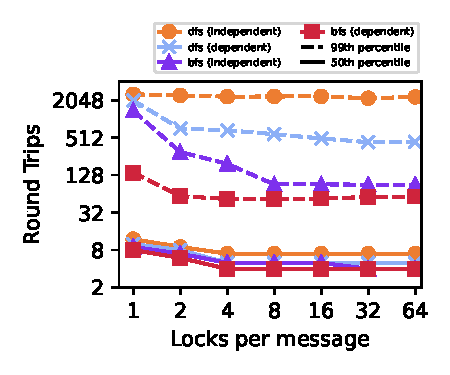
\includegraphics[width=0.99\linewidth]{fig/search_dependence.pdf}
\caption{round trip times required to acquire locks on insert}
             \label{fig:microbenchmarks-b}
\end{figure}

\begin{figure}
\centering
        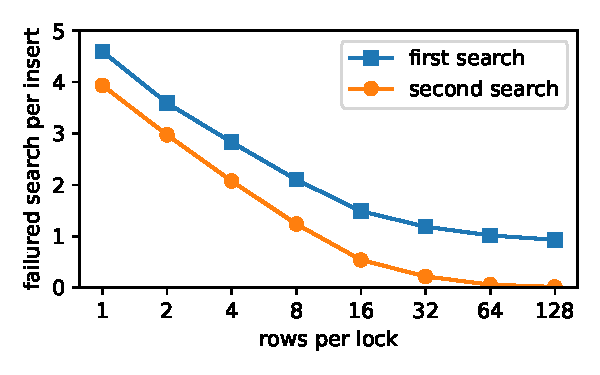
\includegraphics[width=0.99\linewidth]{fig/search_success_lock_size.pdf}
        % \label{fig:hash_factor}
\caption{insert second-search success rate as a function of lock granularity}
             \label{fig:microbenchmarks-c}
\end{figure}

\begin{figure}
\centering
      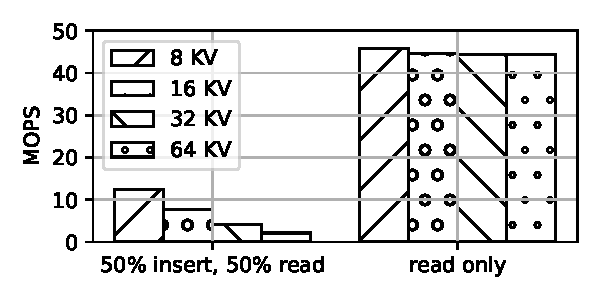
\includegraphics[width=0.99\linewidth]{fig/entry_size.pdf}
\caption{throughput vs. key/value-entry size for YCSB-A (insert) and YCSB-C (read-only) workloads}
             \label{fig:microbenchmarks-d}
\end{figure}

\textbf{Inserts.}
%%
%By default YCSB-A,B,C use updates. RCuckoo's insert
%algorithm is it's most complex and bandwidth intensive
%component. In this section
Despite its complexity, RCuckoo's insert operation remains highly
performant.  To evaluate insert performance we modify YCSB to perform
inserts rather than updates.  Figure~\ref{fig:ycsb_fill} considers
RCuckoo's performance on workloads that exclusively use inserts (rather than
updates), for example in this instance YCSB-A is 50\% insert and 50\%
read. YCSB-W is write only, i.e. a 100\%-insert workload.  Inserts become
more expensive as the table fills, so we prepopulate the table with a varying number of entries and report insert performance as
a function of the table's initial fill factor.
\todo{How long/how many inserts are performed?}

Figure~\ref{fig:ycsb_fill}(a) shows the aggregate throughput of 320
clients across four different workloads as a function of the table's
fill factor.  As the index table fills, cuckoo paths become longer
leading to increased contention and additional bandwidth consumption
from larger covering reads. In each case (except read-only YCSB-C)
RCuckoo's performance declines with fill factor. In the insert-only
YCSB-W case RCuckoo's performance drops from a high of 11.5 MOPS in a
nearly empty table to 4.5 MOPS at a 90\% fill factor.  As a point of
comparison, FUSEE's maximum insert-only performance is 9.1 MOPS on our
testbed, although it is independent of fill factor.  While FUSEE
out-performs RCuckoo at high fill factors, we observe that 
insert-only workloads are rare in
practice~\cite{facebook-memcached}.

\textbf{Latency and overhead.}
We plot operation latency, size, and message counts (in
terms of RDMA packets) as a function of fill factor in
Figure~\ref{fig:ycsb_fill}(b--d).  For comparison, we report
latency values of insert and read operations for the
comparison systems. These values were not collected under
load and represent best-case performance on our testbed.
Read latency is nearly identical for all systems save FUSEE,
as it requires an additional round trip.  Insert times vary:
Clover and Sherman use two-sided RDMA operations for insert
and both need to perform allocations and set up metadata for
the requesting client.  FUSEE is slightly slower, roughly
the same as RCuckoo's best case.  As the table fills,
however, cuckoo paths grow in length causing RCuckoo insert
operations to require additional round trips to find valid
cuckoo paths.  At maximum fill, insert operations take
roughly twice as long as in an empty table. This I/O amplification
is reflected by the increase in both bytes (Figure~\ref{fig:ycsb_fill}(c)) and messages (Figure~\ref{fig:ycsb_fill}(d)) per
operation.  Reads, on the other hand, have roughly
the same cost and performance regardless of fill factor.


% \begin{figure}[t]
%     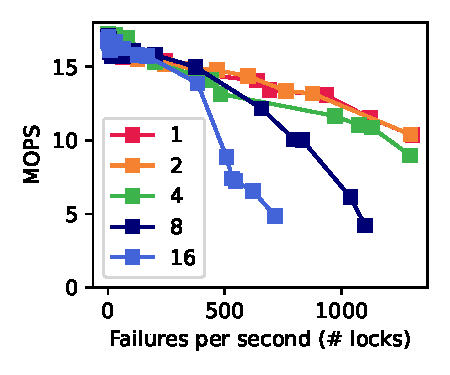
\includegraphics[width=0.99\linewidth]{fig/fault-rate.pdf}
%     \caption{YCSB-A throughput vs. client failure rate.}
%     \label{fig:failure_throughput}
%     \vskip -1em
% \end{figure}

\subsection{Fault tolerance}


RCuckoo runs at nearly full throughput during realistic
failure scenarios and remains functional in the face of
hundreds of failures per second.
%When a client fails while
%holding a lock the lock is stranded and requests for that
%lock will block until after a client times out and reclaims
%the lock.
%%
We emulate client failures by
performing a partial insert operation that randomly truncates the
batch of RDMA operations including lock releases, leaving the table
%. The table
%entries are left
in one of the  states listed in
Section~\ref{sec:table-repair}.
%and locks are left set.
Figure~\ref{fig:microbenchmarks-a} shows that
%illustrates RCuckoo's
%ability to operate at high throughput in the face of
%failures.
%Lock granularity increases the probability that
%multiple clients will block on the same failed lock. Larger
throughput remains high until about 500 client failures per second, at
which point lock granularity begins to play a significant role;
finer-grained locks are easier to recover leading to less throughput
degradation.
%locks have little difference when failures are semi-frequent
%and have a larger impact as hundred of failures occur per
%second.  The performance impact of a few number of failures
%per second is low which is ideal considering that failures
%in RDMA clusters are relatively rare.
As a point of reference, we observe that RDMA itself struggles to handle churn of this magnitude:
%RCuckoo can still operate despite
%thousands of failures per second while
a server can only
establish approximately 1.4~K RDMA connections per second~\cite{xrdma}.
%using state of the art techniques~\cite{xrdma}.

\subsection{Microbenchmarks}
\label{ss:mb}

Having established RCuckoo's superiority over prior systems and
demonstrated its robustness to client failure, we now evaluate the
impact of particular design choices.





% \begin{figure}[t]
%     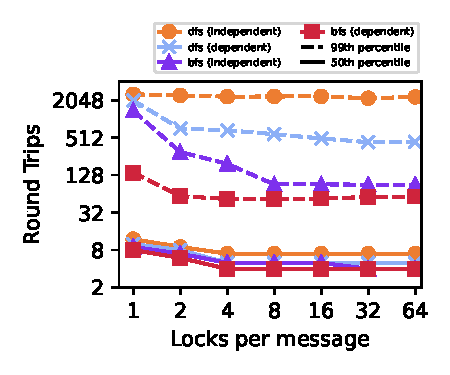
\includegraphics[width=0.99\linewidth]{fig/search_dependence.pdf}
%     \caption{Round trips per insert operation with independent
%     and dependent hashing.  (Note log-scale axes.)}
%     \label{fig:search_dependence}
% \end{figure}
%Hash dependence and search function choice have the highest
%impact on RCuckoo's performance. Dependent hashing reduces
%the probability locks are scattered throughout the table
%which enables RCuckoo to combine lock requests into a few
%masked CAS messages. Simultaneously search function choice
%dramatically affects the length of cuckoo paths.

\textbf{Locality enhancement.}
Figure~\ref{fig:microbenchmarks-b} illustrates the dramatic benefit
RCuckoo extracts from its dependent hashing combined with a BFS
cuckoo-path search strategy.  To focus on longer cuckoo paths, we
prepopulate a 100-M entry table to 85\% and then report both the median
and 99th percentile number of round trips required to insert new
key/value pairs until the table is 95\% full as a function of lock
granularity.  While median performance is on the same order, the
99th-percentile insert takes an order of magnitude fewer round trips
with dependent hashing and BFS as opposed to independent hashing and
DFS as used in prior cuckoo hash
systems~\cite{cuckoo-improvements,pilaf,cuckoo}.  As before
(c.f. Figure~\ref{fig:cuckoo-problems}), performance is similar with
four or more locks per message.

%% We vary the number of locks per message to demonstrate the
%% effect of path length and show why masked cas plays an
%% important role in RCuckoo's performance. We measured both
%% the median, and 99th percentile round trips per request on a
%% table with 100M entries. We fill the table to 85\% and then
%% executed insert operations to 95\%.

%% DFS with no hash dependence has extremely poor performance
%% at it's tail, taking over 2K round trips to complete. Both
%% at it's median and 99th percentile it sees only small
%% benefits from setting multiple locks per request as the
%% locks are scattered throughout the table. DFS with
%% dependence has far lower tail latency, and improves the
%% number of locks which can be acquired per message, however
%% it still constructs long rather than minimum length paths.
%% BFS with dependence provides the best performance and gains
%% the most from setting more locks per request. At 64 locks
%% per request it has 7.5x lower round trips at it's 99th
%% percentile and 4 rather than 5 round trips on average. We
%% found that A* search provided the same minimal path length
%% as DFS with slightly better locality. It's performance
%% against BFS was only superior at fill factors above 95\% and
%% lower elsewhere due to a higher runtime cost on short paths.



% Hash function locality hash a major impact in RCuckoo's
% performance.  Acquiring locks can only be done in a few
% round trips when the locks are clustered together tightly in
% the lock table.  Furthermore, the search function used to
% determine the cuckoo path has a large impact on the locality
% of the locks necessary to lock the path. We evaluate
% dependent hashing and independent hashing as well as random
% and a* search. We measure the number of round trips required
% for each control as a function of the number of locks which
% can be acquired per round trip.

% Figure~\ref{fig:search_dependence} shows the performance
% improvements gained by both locality hashing and A* search.
% In this experiment the table is filled from 0 to 90\% full
% with a YCSB-w workload. We measure the 99th percentile of
% round trips for these workloads. Random search with
% independent hashing leads to a large number of round trips
% as locks are scattered throughout the table. RDMA masked CAS
% operation do little here to reduce the round trips as they
% can rarely acquire more than one lock in a round trip. With
% dependent hashing and random search RDMA CAS operation are
% almost sufficient to reduce round trips, however the absolute
% number of locks required per insert is high which leads to
% greater contention. A* search with dependent hashing has
% cuckoo paths that are both short, and clustered together.



% \label{sec:search_success}
% \begin{figure}[t]
%     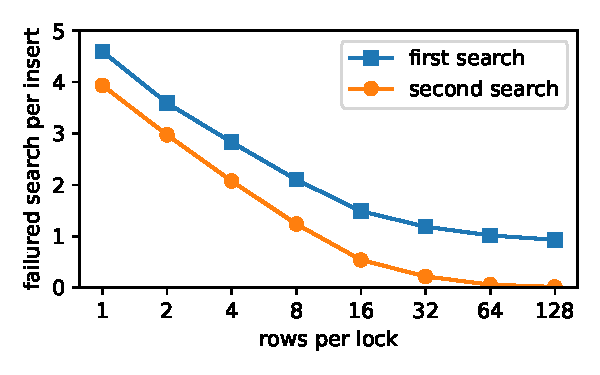
\includegraphics[width=0.99\linewidth]{fig/search_success_lock_size.pdf}
%     \caption{Failure rate of search algorithms vs. lock size under high contention}
%     \label{fig:search_success}
% \end{figure}

\textbf{Secondary search.}
%RCuckoo's two-stage search algorithm is designed to improve
%the probability that an insert will be successful given that
%a clients local cache is out of sync.
To demonstrate the value of RCuckoo's two-stage search strategy we
measure the success rate of the second cuckoo-path search under high
contention.  We prepopulate a small (10-M entry) table up to 85\% and
then have 320 clients concurrently perform insertions (i.e., YCSB-W).
For this experiment only, we flush the client's cache before every
insert, ensuring the initial speculative path will fail unless the entry does
not require cuckooing (unlikely at this fill factor).
%We report the success rate of second   in order to
%maximize cuckoo path length.
Figure~\ref{fig:microbenchmarks-c} plots the success rate of the
second search as a function of lock granularity.  \todo{not sure how
  99th percentile impacts things} Recall that if a second search
fails, RCuckoo clients release their locks and retry the insert
operation using the contents of their cache, so multiple speculative
and secondary searches may be performed.  At one row per lock,
secondary search has limited effectiveness (as the only alternative is
to cuckoo a different set of entries among the same rows), leading to
multiple retries (approaching 4 in the 99th percentile, not shown).
As locks begin to cover additional rows, however, the second search
becomes much more useful.
%% of failure rate of both search stages. The first
%% search is the success rate of a search based entirely on
%% cached information. The second search is the success rate of
%% our restricted search performed after acquiring locks. We
%% measure the response of both as a function of lock size.
%% Given 1 row per lock the failure rate of both searches is
%% over 4 as the local cache is almost always out of sync, and
%% retries are not guaranteed to be synchronized. As lock
%% granularity grows the frequency of second search success
%% drops dramatically. 
At 64 rows per lock the second search
succeeds 95\% of the time.
%even when the cached search fails
%at a rate of 99\% per insert.


%% \subsubsection{Masked CAS}

%% Under contention masked CAS operations provide a significant
%% performance improvement. We measure it's benefit in terms of
%% throughput by comparing it with default CAS. In the
%% default case, when acquiring locks clients set the lock bits
%% for the locks they require and set all other bits in the CAS
%% to 0. If the CAS fails the current state of the lock table
%% over that range is returned as a result to the client and
%% the client tries to acquire their locks again using the
%% updated state of the lock table. Masked compare and swaps
%% are issued with the minimal mask required to set the locks.

%% Figure~\ref{fig:performance_breakdown} shows the improvement
%% gained by masked CAS. Default CAS operations perform better
%% with fewer rows per lock, as the probability of a lock being
%% set within the 64bit range is at its lowest. At higher rows
%% per lock CAS suffers from failed lock acquisitions from both
%% contested locks and due to a lack of synchronization. In
%% contrast masked CAS sees an improvement when two rows per
%% lock are used, as more second search attempts succeed, and
%% only suffers from direct lock contention as the rows per
%% lock increase.


% Figure~\ref{fig:performance_breakdown} plots the sensitivity of
% RCuckoo performance to various parameter settings.


\textbf{Entry size.}
\label{sec:entry_size}
Inlined key/value entries enable single-round-trip
reads, so the larger the entries, the fewer values that
require a second round trip.  However, for a fixed row size,
larger entries imply fewer entries per row, increasing
cuckoo path lengths (when measured in terms of rows).
%,
%impacting insert performance.
%% but larger values must be stored in extents.  % at the
%cost of inflating the bandwidth of % operations. We run a
%50\% read 50\% insert and a read only % workload to
%illustrate the overhead of larger entries.
Figure~\ref{fig:microbenchmarks-d} shows the effect of entry
size on throughput under YCSB-A and YCSB-C (read-only) workloads. Insert is a
bandwidth-limited operation;
%quickly saturates the network bandwidth. At
at 16-B entries link capacity restricts throughput to 8
MOPS. The performance of reads (and updates/deletes, not
shown), are largely unaffected by entry
size.  Hence,
%which have lower bandwidth requirements see very little
%chance in throughput across entry sizes. We suggest that
%known read heavy workloads should use inlined entries as
%reads see a large
read-heavy services may wish to
employ larger entry sizes.
%
%boost in performance. Update operations are similarly
%unaffected by entry size up to 64 bytes. 

% Our design choice
% in embedding KV pairs is motivated by networking trends
% which suggest that 800 GBPS and higher network speeds will
% be available in the coming years. While round trip latency
% is expected to remain largely the same.





%\section{Limitations}
\label{sec:limations}

\subsection{replication and persistance}
At the time of writing Rcuckoo does not support multiple
memory nodes for replication and is not designed for
persistance. No aspect of RCuckoo's algorithm prevents the
use of multiple replicas. As Rcuckoo uses lock based
protection, replicated updates can be broadcast by writes to
each replica prior to releasing locks. Rcuckoo's index is
not designed for persistance. As Rcuckoo is primarily an
index, we see it as compatable with the persistance
strategies of other disaggregated projects. For instance
RCuckoo could easily make use of Clover's persistent extent
algorithm with no changes to RCuckoo's index structure.

\subsection{Client Scalability} RCuckoo's algorithm relies
on the semantics of in order delivery for the correctness of
it's locking and reading algorithms. RDMA NIC's have hard
caps on the number of reliable connections they support
~\todo{(~65k)} these limitations are fundamental to the
cache size on the RDMA NIC~\cite{erpc,faast}, although cache
sizes have steadily increased~\cite{storm}. RDMA unreliable
connections currently do not support one-sided verbs making
them unusable for disaggregated applications.

\section{Conclusion}
\label{sec:conclusion}

In this work we design and implement a lock based cuckoo
hash for remote memory. Using dependent hashing, a carefully
designed locking protocol, and the latest RDMA NIC features
we achieve common case operations of 2 round trips, and
lockless reads in a single round trip. We demonstrate that
these algorithmic advantages lead to better practical
performance by simulating hash table workloads and showing
throughput and latency benefits of up to 2x over state of
the art far memory hash tables.

% \section*{Acknowledgments}

% Thanks for everyone that supported me. Thanks to Pengfei Zuo
% for assistance in replicating results from the original RACE
% paper.


\balance
\vspace{-0.3cm}
{\footnotesize \bibliographystyle{acm}
\bibliography{paper}}
\vspace{-0.5cm}

\end{document}
